\documentclass[oneside,a4paper,12pt]{extreport}

% Font tiếng Việt
\usepackage[T5]{fontenc}
\usepackage[utf8]{inputenc}
\DeclareTextSymbolDefault{\DH}{T1}
\usepackage{times}

% Bookmark tiếng Việt
\usepackage[unicode]{hyperref}

% Chèn hình
\usepackage{graphicx}
\graphicspath{{figures/}{images/}{./}}

% Chèn và định dạng mã nguồn
\usepackage{listings}
\usepackage{xcolor}
\definecolor{codegreen}{rgb}{0,0.6,0}
\definecolor{codegray}{rgb}{0.5,0.5,0.5}
\definecolor{codepurple}{rgb}{0.58,0,0.82}
\definecolor{backcolour}{rgb}{0.95,0.95,0.92}
\lstdefinestyle{mystyle}{
    backgroundcolor=\color{backcolour},
    commentstyle=\color{codegreen},
    keywordstyle=\color{magenta},
    numberstyle=\tiny\color{codegray},
    stringstyle=\color{codepurple},
    basicstyle=\footnotesize,
    breakatwhitespace=false,
    breaklines=true,
    captionpos=b,
    keepspaces=true,
    numbers=left,
    numbersep=5pt,
    showspaces=false,
    showstringspaces=false,
    showtabs=false,
    tabsize=2
}
\lstset{style=mystyle}

% Chèn và định dạng mã giả
\usepackage{amsmath}
\usepackage{algorithm}
\usepackage[noend]{algpseudocode}
\makeatletter
\def\BState{\State\hskip-\ALG@thistlm}
\makeatother

% Bảng biểu
\usepackage{multirow}
\usepackage{booktabs}
\usepackage{array}
\usepackage{longtable}
\newcolumntype{L}[1]{>{\raggedright\let\newline\\\arraybackslash\hspace{0pt}}m{#1}}
\newcolumntype{C}[1]{>{\centering\let\newline\\\arraybackslash\hspace{0pt}}m{#1}}
\newcolumntype{R}[1]{>{\raggedleft\let\newline\\\arraybackslash\hspace{0pt}}m{#1}}

% Hình và vị trí float
\usepackage{float}

% Đổi tên mặc định
\renewcommand{\thefootnote}{[\arabic{footnote}]}
\renewcommand{\chaptername}{Chương}
\renewcommand{\figurename}{Hình}
\renewcommand{\tablename}{Bảng}
\renewcommand{\contentsname}{Mục lục}
\renewcommand{\listfigurename}{Danh sách hình}
\renewcommand{\listtablename}{Danh sách bảng}
\renewcommand{\appendixname}{Phụ lục}

% Định dạng chapter/section theo template
\usepackage{titlesec}
\titleformat{\chapter}
    [display]
    {\normalfont\bfseries\large}{\chaptername\ \thechapter}{10pt}{\huge}
\titlespacing*{\chapter}{0pt}{-10pt}{20pt}

\titleformat{\section}
    {\normalfont\bfseries\large}{\thesection}{1em}{}

\titleformat{\subsection}
    {\normalfont\bfseries\normalsize}{\thesubsection}{1em}{}

% Dãn dòng 1.5
\usepackage{setspace}
\onehalfspacing

% Thụt vào đầu dòng / dãn đoạn
\usepackage{indentfirst}
\setlength{\parskip}{0.6em}
\setlength{\parindent}{0pt}

% Canh lề theo template
\usepackage[
  top=35mm,
  bottom=20mm,
  left=25mm,
  right=25mm,
  footskip=15mm,
  includefoot]{geometry}

% Header/footer
\usepackage{fancyhdr}
\pagestyle{fancy}
\fancyhf{}
\fancyfoot[C]{\thepage}
\begin{document}

%----------------- TRANG BÌA -----------------
\begin{titlepage}
    \centering
    \textbf{\LARGE ĐẠI HỌC QUỐC GIA HÀ NỘI}\\[0.3cm]
    \textbf{\Large TRƯỜNG ĐẠI HỌC CÔNG NGHỆ}\\[2cm]
    \rule{0.8\textwidth}{0.4pt}\\[1cm]

    \IfFileExists{logo.png}{
\includegraphics[width=0.4\textwidth]{logo.png}}{\fbox{\parbox{0.35\textwidth}{\centering Logo UET}}}\\[1cm]

    {\Huge \textbf{BÁO CÁO ĐỒ ÁN}}\\[1.5cm]

    {\LARGE \textbf{Đề tài: Nghiên cứu phát triển hệ thống phát hiện tin giả dựa trên phương pháp tranh biện đa tác tử}}\\[2cm]

    \begin{tabular}{rl}
        \textbf{Sinh viên thực hiện:} & \textbf{Phí Đình Mạnh} -- 23020108 \\
                                      & \textbf{Hoàng Ngọc Hưng} -- 22021170 \\
                                      & \textbf{Trần Trung Kiên} -- 23020087 \\
        \textbf{Giảng viên hướng dẫn:} & TS. Vương Thị Hồng \\
    \end{tabular}

    \vfill
    {\Large Hà Nội, 2026}
\end{titlepage}

% ====================================================================
% LỜI CẢM ƠN
% ====================================================================
\chapter*{Lời cảm ơn}
\addcontentsline{toc}{chapter}{Lời cảm ơn}

Nhóm chúng em xin gửi lời cảm ơn chân thành tới TS. Vương Thị Hồng, giảng viên hướng dẫn đề tài, đã định hướng và hỗ trợ nhóm trong quá trình nghiên cứu, xây dựng và hoàn thiện đồ án. Những góp ý của cô giúp nhóm xác định rõ hơn mục tiêu của bài toán, lựa chọn phương pháp tiếp cận phù hợp và hoàn thiện hệ thống theo hướng có khả năng giải thích tốt hơn.

Nhóm cũng xin cảm ơn Trường Đại học Công nghệ -- Đại học Quốc gia Hà Nội đã tạo môi trường học tập và nghiên cứu thuận lợi, giúp chúng em có cơ hội tiếp cận các kiến thức về trí tuệ nhân tạo, xử lý ngôn ngữ tự nhiên, mô hình ngôn ngữ lớn và các kỹ thuật xây dựng hệ thống phần mềm hiện đại.

Trong quá trình thực hiện, do giới hạn về thời gian, tài nguyên tính toán và kinh nghiệm triển khai hệ thống AI đa tác tử, báo cáo khó tránh khỏi thiếu sót. Nhóm mong nhận được các nhận xét và góp ý để tiếp tục cải thiện hệ thống trong các phiên bản tiếp theo.

% ====================================================================
% LỜI CAM ĐOAN
% ====================================================================
\chapter*{Lời cam đoan}
\addcontentsline{toc}{chapter}{Lời cam đoan}

Nhóm chúng em cam đoan báo cáo đồ án này là kết quả của quá trình tìm hiểu, thiết kế, cài đặt và thực nghiệm do nhóm thực hiện dưới sự hướng dẫn của giảng viên. Các nội dung tham khảo từ tài liệu, công cụ, thư viện hoặc bộ dữ liệu bên ngoài đều được sử dụng với mục đích học thuật và được trình bày trong phạm vi phù hợp của báo cáo.

Các kết quả thực nghiệm, nhận xét và phân tích trong báo cáo được xây dựng dựa trên quá trình chạy thử hệ thống, kiểm tra nhật ký đầu ra và so sánh với nhãn của bộ dữ liệu đánh giá. Nhóm không sao chép nguyên văn kết quả của công trình khác để thay thế cho kết quả thực hiện của mình.

% ====================================================================
% TÓM TẮT
% ====================================================================
\chapter*{Tóm tắt}
\addcontentsline{toc}{chapter}{Tóm tắt}

Sự phát triển của mạng xã hội và các nền tảng chia sẻ nội dung khiến tin giả, tin sai lệch và thông tin thiếu kiểm chứng có khả năng lan truyền với tốc độ rất lớn. Trong khi đó, các mô hình ngôn ngữ lớn có thể hỗ trợ phân tích văn bản và kiểm chứng thông tin, nhưng nếu sử dụng một mô hình đơn lẻ thì hệ thống dễ gặp các vấn đề như ảo giác thông tin, trả lời thiếu căn cứ, thiếu khả năng phản biện và khó giải thích vì sao đưa ra kết luận.

Đồ án này xây dựng một hệ thống phát hiện tin giả dựa trên phương pháp \textit{Tranh biện đa tác tử} (MAD). Thay vì yêu cầu một mô hình duy nhất đưa ra phán quyết trực tiếp, hệ thống tổ chức một quy trình tranh luận nhiều vòng giữa các tác tử có vai trò khác nhau. Tác tử bảo vệ cố gắng bảo vệ tính đúng đắn của bản tin, Tác tử phản biện tìm các điểm sai lệch hoặc thiếu căn cứ, Bộ đánh giá nguồn đánh giá độ tin cậy của nguồn bằng chứng, và Tác tử phán quyết tổng hợp toàn bộ quá trình để đưa ra điểm chân thực cuối cùng.

Hệ thống được triển khai bằng Python, sử dụng LangGraph để điều phối luồng xử lý dạng đồ thị trạng thái, LangChain để giao tiếp với mô hình ngôn ngữ lớn, Tavily và Wikipedia để thu thập bằng chứng, cùng Gradio cho giao diện trình diễn. Ngoài chế độ tìm kiếm mở trên web, hệ thống còn hỗ trợ chế độ không tìm kiếm, trong đó toàn bộ lập luận được giới hạn trong ngữ cảnh đầu vào. Chế độ này đặc biệt phù hợp cho đánh giá trên bộ dữ liệu FEVER, nơi mỗi nhận định có bằng chứng Wikipedia đi kèm.

Kết quả thực nghiệm cho thấy cách tiếp cận MAD có khả năng cải thiện độ chính xác so với việc hỏi trực tiếp một mô hình ngôn ngữ đơn lẻ. Quan trọng hơn, hệ thống không chỉ trả về nhãn đúng/sai, mà còn cung cấp lịch sử tranh luận, nguồn bằng chứng và các luận điểm quyết định, giúp quá trình kiểm chứng trở nên minh bạch và dễ phân tích hơn.

\tableofcontents
\listoffigures
\listoftables
\newpage

% ====================================================================
% DANH MỤC TỪ VIẾT TẮT
% ====================================================================
\chapter*{Danh mục từ viết tắt}
\addcontentsline{toc}{chapter}{Danh mục từ viết tắt}

\begin{longtable}{|p{1.2cm}|p{2.8cm}|p{4.6cm}|p{5.2cm}|}
\hline
\textbf{STT} & \textbf{Từ viết tắt} & \textbf{Từ đầy đủ tiếng Anh} & \textbf{Nghĩa tiếng Việt} \\
\hline
1 & API & Application Programming Interface & Giao diện lập trình ứng dụng \\
\hline
2 & AI & Artificial Intelligence & Trí tuệ nhân tạo \\
\hline
3 & LLM & Large Language Model & Mô hình ngôn ngữ lớn \\
\hline
4 & MAD & Multi-Agent Debate & Tranh biện đa tác tử \\
\hline
5 & RAG & Retrieval-Augmented Generation & Sinh văn bản tăng cường truy xuất \\
\hline
6 & FEVER & Fact Extraction and Verification & Bộ dữ liệu kiểm chứng nhận định dựa trên bằng chứng \\
\hline
7 & JSON & JavaScript Object Notation & Định dạng trao đổi dữ liệu có cấu trúc \\
\hline
8 & UI & User Interface & Giao diện người dùng \\
\hline
9 & CLI & Command Line Interface & Giao diện dòng lệnh \\
\hline
10 & HTTP & HyperText Transfer Protocol & Giao thức truyền tải siêu văn bản \\
\hline
\end{longtable}


% ====================================================================
% CHƯƠNG 1
% ====================================================================
\chapter{Giới thiệu đề tài}

\section{Bối cảnh và động lực}

Trong bối cảnh xã hội số, thông tin được tạo ra, chia sẻ và tiêu thụ với tốc độ rất lớn. Mạng xã hội, nền tảng video ngắn, diễn đàn trực tuyến và các trang tin tổng hợp giúp người dùng tiếp cận tin tức gần như theo thời gian thực. Tuy nhiên, cùng với lợi ích về tốc độ lan truyền, môi trường này cũng tạo điều kiện cho tin giả, tin sai lệch và các nội dung gây hiểu nhầm phát tán rộng rãi. Một tiêu đề được viết theo hướng giật gân, một đoạn trích thiếu ngữ cảnh hoặc một tuyên bố chưa được kiểm chứng có thể nhanh chóng được chia sẻ lại bởi nhiều người trước khi được xác minh.

Tin giả không chỉ là vấn đề kỹ thuật của xử lý văn bản \cite{vosoughi2018spread}. Nó còn liên quan tới nhận thức xã hội, hành vi người dùng, độ tin cậy của nguồn tin và cách thông tin được diễn giải. Trong các lĩnh vực như y tế, chính trị, tài chính hoặc an toàn cộng đồng, một thông tin sai có thể dẫn tới quyết định sai. Ví dụ, một tin đồn không chính xác về thuốc, vaccine hoặc chính sách công có thể ảnh hưởng tới hành vi của một cộng đồng lớn. Do đó, bài toán phát hiện tin giả cần được tiếp cận như một bài toán kiểm chứng thông tin có bằng chứng, thay vì chỉ là bài toán phân loại văn bản đơn giản.

Các phương pháp phát hiện tin giả truyền thống thường khai thác một hoặc nhiều nhóm đặc trưng như đặc trưng ngôn ngữ, đặc trưng người đăng, đặc trưng mạng lan truyền hoặc đặc trưng tương tác của người dùng. Những phương pháp này có giá trị trong các bối cảnh dữ liệu ổn định và có nhãn đầy đủ, nhưng thường gặp khó khăn khi nội dung mới xuất hiện liên tục, khi nhận định liên quan tới sự kiện ngoài tập huấn luyện hoặc khi thông tin sai được viết bằng văn phong tự nhiên, thuyết phục. Ngoài ra, nhiều hệ thống phân loại chỉ trả về nhãn dự đoán mà không chỉ ra rõ bằng chứng nào được dùng để đưa ra kết luận.

Sự phát triển của mô hình ngôn ngữ lớn mở ra một hướng tiếp cận mới cho bài toán kiểm chứng thông tin. Các mô hình này có khả năng hiểu ngữ cảnh, phân tích lập luận, tóm tắt nội dung và sinh giải thích bằng ngôn ngữ tự nhiên. Tuy nhiên, nếu chỉ hỏi trực tiếp một mô hình duy nhất rằng một bản tin là thật hay giả, hệ thống vẫn tồn tại nhiều rủi ro: mô hình có thể ảo giác, có thể bỏ qua chi tiết nhỏ nhưng quan trọng, có thể bị ảnh hưởng bởi cách đặt câu hỏi, hoặc đưa ra câu trả lời có vẻ tự tin dù thiếu bằng chứng. Đây là hạn chế nghiêm trọng đối với một hệ thống kiểm chứng thông tin, nơi tính đúng đắn, khả năng giải thích và khả năng truy vết đều rất quan trọng.

Từ những vấn đề trên, đồ án lựa chọn hướng tiếp cận \textit{Tranh biện đa tác tử} (MAD). Thay vì để một mô hình đơn lẻ đưa ra kết luận trực tiếp, hệ thống tổ chức một quá trình tranh luận có cấu trúc giữa nhiều tác tử chuyên biệt. Một tác tử đóng vai trò bảo vệ tính đúng đắn của bản tin, một tác tử đóng vai trò phản biện, một thành phần đánh giá độ tin cậy của nguồn bằng chứng, và một tác tử cuối cùng tổng hợp toàn bộ quá trình để đưa ra phán quyết. Cách tiếp cận này giúp hệ thống không chỉ trả lời ``đúng'' hay ``sai'', mà còn cho thấy thông tin đã được kiểm tra qua những lập luận nào, nguồn nào có trọng lượng, và vì sao kết luận cuối cùng được hình thành.

\section{Các hướng tiếp cận liên quan}

Trước khi xây dựng hệ thống MAD, cần nhìn nhận bài toán phát hiện tin giả trong tương quan với một số hướng tiếp cận phổ biến. Mỗi hướng có ưu điểm riêng, nhưng cũng tồn tại những giới hạn khiến chúng chưa đáp ứng đầy đủ yêu cầu của một hệ thống kiểm chứng có giải thích.

Nhóm phương pháp thứ nhất là các mô hình phân loại dựa trên đặc trưng văn bản. Các phương pháp này xem một bản tin hoặc một tiêu đề như một mẫu dữ liệu đầu vào, sau đó trích xuất đặc trưng ngôn ngữ để dự đoán nhãn thật/giả. Đặc trưng có thể là n-gram, TF-IDF, embedding hoặc biểu diễn ngữ nghĩa từ các mô hình học sâu. Ưu điểm của hướng này là quy trình huấn luyện và suy luận tương đối rõ ràng, tốc độ nhanh và có thể đạt kết quả tốt trên bộ dữ liệu cố định. Tuy nhiên, nhược điểm là mô hình dễ học các dấu hiệu bề mặt của tập dữ liệu thay vì thật sự kiểm chứng nội dung. Khi gặp một nhận định mới cần tri thức ngoài, mô hình phân loại thuần túy thường không có khả năng tự tìm bằng chứng.

Nhóm phương pháp thứ hai khai thác hành vi lan truyền và thông tin mạng xã hội. Thay vì chỉ nhìn vào nội dung, hệ thống xem xét ai là người đăng, tốc độ lan truyền, cấu trúc chia sẻ, phản ứng của người dùng hoặc mối quan hệ giữa các tài khoản. Hướng này hữu ích khi dữ liệu xã hội đầy đủ, đặc biệt với các tin lan truyền mạnh. Tuy nhiên, nó ít phù hợp với bài toán kiểm chứng một nhận định độc lập, nơi hệ thống chỉ nhận được một đoạn văn bản đầu vào mà không có dữ liệu lan truyền đi kèm. Ngoài ra, một thông tin đúng nhưng gây tranh cãi cũng có thể có hành vi lan truyền bất thường, khiến việc dựa vào tín hiệu xã hội trở nên không đủ chắc chắn.

Nhóm phương pháp thứ ba là các hệ thống kiểm chứng thông tin dựa trên truy xuất bằng chứng. Với hướng này, hệ thống tìm các tài liệu liên quan, sau đó so sánh nhận định với bằng chứng để xác định nhận định được hỗ trợ hay bị phản bác. Đây là hướng gần với mục tiêu của đồ án nhất vì nó nhấn mạnh vai trò của bằng chứng. Tuy nhiên, nếu chỉ sử dụng một mô hình suy luận duy nhất sau bước truy xuất, hệ thống vẫn có thể bỏ sót phản biện hoặc diễn giải bằng chứng theo một chiều. Vì vậy, đồ án kết hợp truy xuất bằng chứng với cơ chế tranh luận đa tác tử để tăng khả năng đối soát.

Nhóm phương pháp thứ tư là sử dụng trực tiếp mô hình ngôn ngữ lớn. Cách này đơn giản, linh hoạt và dễ triển khai: người dùng đưa nhận định vào chỉ dẫn và yêu cầu mô hình trả lời đúng/sai kèm giải thích. Tuy nhiên, đây cũng là cách có rủi ro cao nhất nếu không có cơ chế kiểm soát. Mô hình có thể tạo ra nguồn không tồn tại, đánh giá quá tự tin, hoặc không phân biệt rõ giữa tri thức phổ thông, suy luận logic và bằng chứng đã được xác thực. Đối với một hệ thống phục vụ kiểm chứng, việc thiếu cơ chế phản biện và thiếu cấu trúc lưu vết là một hạn chế lớn.

Từ việc phân tích các hướng trên, đồ án định vị hệ thống MAD như một giải pháp kết hợp. Hệ thống tận dụng khả năng ngôn ngữ và suy luận của LLM, kết hợp với truy xuất bằng chứng bên ngoài, đồng thời bổ sung cơ chế tranh luận đối kháng để giảm sự phụ thuộc vào một câu trả lời đơn lẻ. Đây không phải là một bộ phân loại đơn giản, mà là một quy trình kiểm chứng nhiều bước, trong đó mỗi kết luận cuối cùng được hình thành từ quá trình tìm kiếm, lập luận, phản biện và tổng hợp.

\section{Bài toán đặt ra}

Bài toán của đồ án là xây dựng một hệ thống có khả năng tiếp nhận một bản tin, tiêu đề hoặc nhận định dạng văn bản và đưa ra đánh giá về mức độ chân thực của nội dung đó. Điểm quan trọng là hệ thống không chỉ cần dự đoán nhãn đúng/sai, mà phải cung cấp được quá trình lập luận dẫn tới kết luận. Với bài toán phát hiện tin giả trong bối cảnh sử dụng LLM, một phán quyết chỉ thực sự có giá trị khi nó đi kèm với bằng chứng, lý do và khả năng truy vết.

Về mặt hình thức, đầu vào chính của hệ thống là một văn bản cần kiểm chứng. Văn bản này có thể là một nhận định ngắn, một tiêu đề tin tức, một đoạn mô tả sự kiện hoặc một phát biểu được trích từ bài viết. Trong một số trường hợp, hệ thống có thể nhận thêm ngữ cảnh ban đầu, chẳng hạn đoạn bằng chứng Wikipedia hoặc tài liệu nội bộ. Ngữ cảnh này đặc biệt quan trọng trong chế độ không tìm kiếm, khi hệ thống bị giới hạn trong nguồn thông tin đã được cung cấp và không được truy xuất thêm dữ liệu từ bên ngoài.

Đầu ra của hệ thống gồm nhiều lớp thông tin. Lớp đầu tiên là điểm chân thực \texttt{truth\_score}, biểu diễn mức độ hệ thống đánh giá nhận định là đúng. Lớp thứ hai là phần giải thích cuối cùng, trong đó tác tử phán quyết nêu các điểm quyết định quan trọng nhất. Lớp thứ ba là lịch sử tranh luận, bao gồm các nhận định ban đầu, phản biện, hành động bảo vệ và bằng chứng được trích dẫn qua từng vòng. Lớp thứ tư là kho bằng chứng, tức tập nguồn đã được hệ thống sử dụng hoặc xem xét trong quá trình phân tích.

Có thể xem bài toán gồm ba bài toán con liên kết chặt chẽ với nhau. Bài toán con thứ nhất là truy xuất và tổ chức bằng chứng: hệ thống cần tìm hoặc tiếp nhận các nguồn liên quan, gán định danh và đánh giá mức độ đáng tin. Bài toán con thứ hai là lập luận đối kháng: các tác tử cần xây dựng luận điểm, phản biện luận điểm của phía đối lập và bảo vệ các nhận định còn giá trị. Bài toán con thứ ba là tổng hợp phán quyết: hệ thống cần đánh giá toàn bộ quá trình tranh luận để đưa ra kết luận cuối cùng. Ba bài toán con này tạo thành luồng xử lý chính của hệ thống MAD.

\section{Mục tiêu đồ án}

Mục tiêu tổng quát của đồ án là nghiên cứu và xây dựng một hệ thống phát hiện tin giả dựa trên mô hình tranh luận đa tác tử, có khả năng kết hợp giữa truy xuất bằng chứng, lập luận đối kháng và phán quyết có giải thích. Hệ thống hướng tới việc nâng cao tính minh bạch của quá trình kiểm chứng, đồng thời giảm sự phụ thuộc vào câu trả lời trực tiếp của một mô hình ngôn ngữ đơn lẻ.

Về mặt thiết kế hệ thống, đồ án đặt mục tiêu xây dựng một kiến trúc gồm nhiều tác tử với vai trò chuyên biệt. Tác tử bảo vệ có nhiệm vụ bảo vệ tính đúng đắn của thông tin đầu vào. Tác tử phản biện có nhiệm vụ tìm điểm sai lệch, thiếu căn cứ hoặc mâu thuẫn. Bộ đánh giá nguồn đánh giá chất lượng nguồn bằng chứng. Tác tử phán quyết tổng hợp toàn bộ tranh luận và đưa ra kết luận cuối cùng. Việc phân vai này giúp quá trình suy luận trở nên rõ ràng hơn, đồng thời tạo điều kiện để phân tích từng bước nếu hệ thống đưa ra kết quả sai.

Về mặt điều phối, đồ án xây dựng luồng xử lý nhiều vòng bằng LangGraph. Hệ thống cần duy trì trạng thái qua các vòng tranh luận, bao gồm nguồn bằng chứng, danh sách truy vấn đã thực hiện, lịch sử tranh luận, các nhận định đang được theo dõi và kết quả cuối cùng. Cách tổ chức bằng đồ thị trạng thái giúp hệ thống có thể lặp lại một chuỗi xử lý phức tạp mà vẫn đảm bảo các dữ liệu trung gian được quản lý nhất quán.

Về mặt dữ liệu và bằng chứng, đồ án thiết kế kho bằng chứng dùng chung cho các tác tử. Mỗi nguồn được gán mã định danh, nội dung trích xuất, miền nguồn, độ liên quan và điểm tin cậy. Khi tác tử đưa ra lập luận, nguồn được trích dẫn thông qua mã định danh này. Cơ chế này giúp lập luận có căn cứ hơn và giúp tác tử phán quyết kiểm tra xem một phát biểu có thực sự được hỗ trợ bởi nguồn hay không.

Về mặt quản lý lập luận, đồ án thiết kế bộ quản lý nhận định để theo dõi các nhận định của tác tử bảo vệ và tác tử phản biện qua nhiều vòng. Thay vì để các tác tử sinh văn bản tự do, hệ thống yêu cầu mỗi nhận định có định danh như D1, D2, C1, C2. Ở các vòng sau, phản biện hoặc bảo vệ phải hướng tới một nhận định cụ thể. Cách này giúp tránh việc tranh luận lan man, đồng thời tạo ra một cấu trúc lập luận có thể phân tích sau khi hệ thống kết thúc.

Về mặt đánh giá, đồ án xây dựng quy trình thực nghiệm so sánh hệ thống MAD với cách hỏi trực tiếp mô hình nền đơn lẻ trên bộ dữ liệu FEVER. Mục tiêu không chỉ là đo độ chính xác, mà còn phân tích xem MAD cải thiện ở đâu, thất bại trong trường hợp nào và những thất bại đó phản ánh hạn chế nào của hệ thống.

\section{Phạm vi thực hiện}

Trong phạm vi đồ án, hệ thống tập trung vào kiểm chứng thông tin dạng văn bản. Các dạng dữ liệu khác như hình ảnh, video, âm thanh hoặc dữ liệu mạng xã hội đa phương tiện chưa được xử lý trực tiếp. Đây là lựa chọn phù hợp với mục tiêu chính của đồ án: xây dựng và đánh giá cơ chế tranh luận đa tác tử cho nhận định dạng văn bản trước khi mở rộng sang các loại dữ liệu phức tạp hơn.

Hệ thống không thực hiện fine-tuning mô hình ngôn ngữ. Thay vào đó, các mô hình được sử dụng thông qua API tương thích OpenAI và có thể thay đổi bằng cấu hình môi trường. Cách tiếp cận này giúp đồ án tập trung vào thiết kế kiến trúc, điều phối tác tử, quản lý bằng chứng và đánh giá hệ thống, thay vì tập trung vào huấn luyện mô hình nền. Đây cũng là hướng triển khai thực tế trong nhiều ứng dụng LLM hiện nay, nơi khả năng phối hợp công cụ và thiết kế quy trình thường quan trọng không kém việc lựa chọn mô hình.

Về nguồn bằng chứng, hệ thống hỗ trợ hai chế độ vận hành. Ở chế độ tìm kiếm, hệ thống sử dụng Tavily và Wikipedia để thu thập nguồn liên quan. Chế độ này phù hợp với các tình huống kiểm chứng mở, khi người dùng nhập một bản tin mới và hệ thống cần tự tìm tài liệu hỗ trợ hoặc phản bác. Ở chế độ không tìm kiếm, hệ thống chỉ sử dụng ngữ cảnh đầu vào, phù hợp cho bộ đánh giá hoặc các trường hợp cần kiểm chứng trong phạm vi tài liệu đã được kiểm soát.

Về đánh giá, trọng tâm của báo cáo là bộ dữ liệu FEVER ở dạng nhị phân SUPPORTS/REFUTES. FEVER phù hợp với đồ án vì mỗi nhận định có bằng chứng Wikipedia liên quan, giúp đánh giá năng lực suy luận dựa trên bằng chứng. Một số kịch bản cho GossipCop và TruthfulQA được xây dựng nhằm chuẩn bị cho các hướng thử nghiệm mở rộng, nhưng phần thực nghiệm chính trong báo cáo tập trung vào FEVER để đảm bảo tính nhất quán và khả năng phân tích sâu.

\section{Đóng góp chính của đồ án}

Đồ án có một số đóng góp chính. Thứ nhất, đồ án xây dựng một kiến trúc kiểm chứng tin giả dựa trên tranh luận đa tác tử, trong đó quá trình kết luận được chia thành nhiều vai trò và nhiều bước rõ ràng. Thứ hai, hệ thống kết hợp được truy xuất bằng chứng, chấm điểm nguồn và quản lý lập luận trong cùng một luồng xử lý. Thứ ba, đồ án thiết kế bộ quản lý nhận định để theo dõi các nhận định qua nhiều vòng, giúp quá trình tranh luận có cấu trúc và có khả năng truy vết. Thứ tư, hệ thống hỗ trợ cả chế độ tìm kiếm mở và chế độ không tìm kiếm, cho phép vừa trình diễn trên tin tức mới vừa đánh giá trên bộ đánh giá có ngữ cảnh chuẩn. Thứ năm, đồ án xây dựng quy trình thực nghiệm so sánh MAD với mô hình nền đơn lẻ và phân tích các trường hợp thất bại để rút ra nhận xét về ưu điểm, hạn chế của hướng tiếp cận.

Các đóng góp này cho thấy trọng tâm của đồ án không nằm ở việc tạo thêm một mô hình phân loại tin giả, mà nằm ở việc xây dựng một quy trình kiểm chứng có cấu trúc, có bằng chứng và có khả năng giải thích. Đây là điểm khác biệt quan trọng khi ứng dụng LLM vào các bài toán yêu cầu độ tin cậy cao.

\section{Cấu trúc báo cáo}

Báo cáo được tổ chức thành bảy chương. Chương 1 giới thiệu bối cảnh, các hướng tiếp cận liên quan, bài toán, mục tiêu, phạm vi và đóng góp của đồ án. Chương 2 trình bày cơ sở lý thuyết và các công nghệ được sử dụng, bao gồm kiểm chứng thông tin, hạn chế của LLM đơn lẻ, truy xuất bằng chứng và tranh biện đa tác tử. Chương 3 phân tích và thiết kế kiến trúc hệ thống, tập trung vào luồng xử lý, các tác tử, trạng thái dùng chung và hai chế độ vận hành. Chương 4 mô tả quá trình cài đặt và triển khai. Chương 5 trình bày phương pháp thực nghiệm và quy trình đánh giá. Chương 6 phân tích kết quả thực nghiệm và các trường hợp thất bại tiêu biểu. Chương 7 tổng kết đóng góp, hạn chế và hướng phát triển tiếp theo.

% ====================================================================
% CHƯƠNG 2
% ====================================================================

\chapter{Cơ sở lý thuyết và công nghệ sử dụng}

\section{Bài toán phát hiện tin giả và kiểm chứng thông tin}

Phát hiện tin giả là bài toán xác định một nội dung thông tin có phản ánh đúng sự thật hay không. Ở mức đơn giản, bài toán này có thể được mô hình hóa như một bài toán phân loại văn bản, trong đó hệ thống nhận vào một bản tin và trả về nhãn như thật, giả hoặc không chắc chắn. Tuy nhiên, trong bối cảnh thực tế, cách nhìn này là chưa đầy đủ. Một bản tin có thể chứa nhiều phát biểu nhỏ, trong đó có phát biểu đúng, phát biểu sai, phát biểu thiếu ngữ cảnh hoặc phát biểu chưa đủ bằng chứng để kết luận. Vì vậy, phát hiện tin giả cần được đặt gần hơn với bài toán kiểm chứng thông tin, tức là đánh giá từng nhận định dựa trên bằng chứng cụ thể.

Khác với phân loại văn bản thông thường, kiểm chứng thông tin không chỉ quan tâm tới kết quả cuối cùng mà còn quan tâm tới quá trình đi đến kết quả đó. Một mô hình phân loại có thể dựa trên các dấu hiệu bề mặt như cách dùng từ, độ giật gân của tiêu đề hoặc phong cách viết để dự đoán tin thật/giả. Cách này có thể hiệu quả trên một tập dữ liệu nhất định, nhưng không đảm bảo rằng mô hình thật sự hiểu và kiểm chứng nội dung. Trong khi đó, một hệ thống kiểm chứng thông tin cần trả lời các câu hỏi sâu hơn: nhận định đang nói về sự kiện nào, bằng chứng nào liên quan, nguồn nào đáng tin, nhận định được nguồn hỗ trợ hay bị nguồn phản bác, và phần nào của nhận định là nguyên nhân dẫn đến kết luận.

Một quy trình kiểm chứng thông tin thường gồm ba giai đoạn. Giai đoạn thứ nhất là nhận diện nội dung cần kiểm chứng. Hệ thống phải hiểu được nhận định hoặc bản tin đang đề cập tới các thực thể nào, mốc thời gian nào, quan hệ nào và sự kiện nào. Đây là bước quan trọng vì nhiều tin giả không sai hoàn toàn, mà sai ở một chi tiết nhỏ như con số, thời điểm, vai trò của nhân vật hoặc phạm vi áp dụng của một kết luận. Giai đoạn thứ hai là thu thập hoặc tiếp nhận bằng chứng. Bằng chứng có thể đến từ tài liệu được cung cấp sẵn, nguồn tri thức mở, trang tin uy tín hoặc kết quả tìm kiếm web. Giai đoạn thứ ba là suy luận trên bằng chứng để xác định nhận định được hỗ trợ, bị phản bác hay chưa đủ căn cứ.

Trong các bộ dữ liệu kiểm chứng thông tin, bài toán thường được biểu diễn ở mức nhận định. Một nhận định là một phát biểu có thể kiểm chứng, ví dụ một người giữ chức vụ nào đó, một sự kiện xảy ra tại một thời điểm cụ thể, hoặc một con số thống kê thuộc về một phạm vi nhất định. Một số hệ thống sử dụng ba nhãn phổ biến: \textit{supports}, \textit{refutes} và \textit{not enough information}. Trong đồ án này, để phục vụ đánh giá rõ ràng và phù hợp với thiết lập thực nghiệm, nhóm sử dụng biến thể nhị phân của FEVER, trong đó SUPPORTS được ánh xạ thành 1.0 và REFUTES được ánh xạ thành 0.0. Cách thiết lập này giúp so sánh trực tiếp giữa mô hình nền đơn lẻ và hệ thống MAD thông qua các chỉ số như độ chính xác, độ chính xác dương, độ bao phủ và F1-score.

Một yêu cầu quan trọng khác của kiểm chứng thông tin là tính giải thích. Trong nhiều ứng dụng, chỉ biết một bản tin bị đánh giá là sai là chưa đủ. Người dùng cần biết bản tin sai vì lý do nào: do không có nguồn xác nhận, do nguồn phản bác trực tiếp, do đánh tráo khái niệm, do suy luận quá mức từ dữ kiện có thật, hay do nhầm lẫn giữa một tập hợp tổng và một tập hợp con. Vì vậy, hệ thống cần tạo ra một dạng \textit{kiểm tra truy vết trail}, tức là chuỗi thông tin cho phép truy vết quá trình suy luận. Đây cũng là một trong những lý do chính khiến đồ án lựa chọn kiến trúc nhiều bước thay vì một bộ phân loại đơn giản.

Từ góc nhìn thiết kế hệ thống, phát hiện tin giả trong đồ án được xem như một quy trình gồm bốn năng lực chính. Thứ nhất là năng lực truy xuất và tổ chức bằng chứng. Thứ hai là năng lực đánh giá chất lượng nguồn. Thứ ba là năng lực xây dựng và phản biện lập luận. Thứ tư là năng lực tổng hợp phán quyết cuối cùng. Một hệ thống chỉ mạnh ở một trong bốn năng lực này vẫn có thể đưa ra kết quả thiếu ổn định. Ví dụ, truy xuất được nguồn tốt nhưng suy luận kém vẫn có thể kết luận sai; lập luận tốt nhưng nguồn yếu vẫn thiếu độ tin cậy; tác tử phán quyết mạnh nhưng không có lịch sử tranh luận rõ ràng thì khó giải thích. Do đó, hệ thống MAD được thiết kế để phối hợp cả bốn năng lực trong cùng một luồng xử lý.

\section{Hạn chế của mô hình ngôn ngữ đơn lẻ}

Mô hình ngôn ngữ lớn có khả năng xử lý ngôn ngữ tự nhiên rất mạnh. Khi được yêu cầu đánh giá một nhận định, mô hình có thể phân tích ngữ nghĩa, đưa ra giải thích mạch lạc và thậm chí chỉ ra một số điểm bất hợp lý trong nội dung. Tuy nhiên, nếu sử dụng một mô hình đơn lẻ như một bộ phán quyết trực tiếp, hệ thống vẫn gặp nhiều hạn chế về độ tin cậy, khả năng cập nhật thông tin và khả năng kiểm soát quá trình suy luận.

Hạn chế đầu tiên là hiện tượng ảo giác thông tin. Mô hình ngôn ngữ được huấn luyện để dự đoán và sinh chuỗi văn bản có xác suất cao, không phải để đảm bảo mọi phát biểu đều có nguồn xác thực. Do đó, trong một số trường hợp, mô hình có thể tạo ra câu trả lời nghe hợp lý nhưng không dựa trên bằng chứng cụ thể. Với các tác vụ sáng tạo hoặc hội thoại thông thường, lỗi này có thể chấp nhận ở mức nhất định. Nhưng với kiểm chứng thông tin, một phát biểu không có căn cứ vẫn được trình bày tự tin có thể làm sai lệch toàn bộ kết quả đánh giá.

Hạn chế thứ hai là kiến thức tĩnh và không đầy đủ. Mô hình chỉ phản ánh tri thức được học trong quá trình huấn luyện, bị giới hạn bởi thời điểm cắt dữ liệu, phạm vi dữ liệu và chất lượng dữ liệu huấn luyện. Với tin tức, nhiều sự kiện mới xuất hiện sau thời điểm huấn luyện hoặc thay đổi theo thời gian. Một mô hình không có truy xuất bên ngoài có thể không biết thông tin mới, hoặc tệ hơn là suy đoán dựa trên các mẫu đã học. Vì vậy, một hệ thống kiểm chứng cần có cơ chế đưa bằng chứng mới vào quá trình suy luận thay vì chỉ dựa vào tri thức nội tại.

Hạn chế thứ ba là thiếu cơ chế phản biện nội tại. Khi được hỏi trực tiếp, mô hình thường sinh ra một câu trả lời tuyến tính: kết luận trước, sau đó giải thích theo hướng củng cố kết luận đó. Nếu câu trả lời ban đầu bị lệch, phần giải thích phía sau có thể trở thành một dạng hợp thức hóa cho kết luận sai. Một mô hình đơn lẻ không có vai trò đối lập chủ động đặt câu hỏi, tấn công vào điểm yếu, kiểm tra từng chi tiết hoặc yêu cầu bằng chứng cụ thể. Điều này đặc biệt nguy hiểm với các nhận định mơ hồ, nhận định chứa số liệu, nhận định dùng thuật ngữ dễ đánh tráo hoặc nhận định cần phân biệt giữa nhiều nguồn gần giống nhau.

Hạn chế thứ tư là độ nhạy với cách đặt chỉ dẫn. Cùng một nhận định nhưng nếu được hỏi bằng các cách khác nhau, mô hình có thể đưa ra mức độ chắc chắn khác nhau hoặc nhấn mạnh các khía cạnh khác nhau. Trong một hệ thống kiểm chứng nghiêm túc, kết quả không nên phụ thuộc quá nhiều vào một câu hỏi đơn lẻ. Cần có một quy trình buộc mô hình phải đi qua các bước ổn định hơn: xem bằng chứng, xây dựng luận điểm, phản biện luận điểm, lưu lịch sử và tổng hợp kết luận.

Hạn chế thứ năm là thiếu khả năng truy vết nếu chỉ dùng một lần gọi mô hình. Khi mô hình trả lời trực tiếp rằng nhận định đúng hay sai, người dùng khó biết trong quá trình suy luận mô hình đã cân nhắc những khả năng nào, bỏ qua bằng chứng nào, hay có nhầm lẫn giữa các khái niệm gần nhau hay không. Ngay cả khi mô hình đưa ra giải thích, phần giải thích đó vẫn là sản phẩm sinh ra sau cùng, không nhất thiết phản ánh một quy trình kiểm tra có cấu trúc. Điều này làm giảm khả năng phân tích lỗi và cải tiến hệ thống.

Những hạn chế trên không có nghĩa là mô hình ngôn ngữ lớn không phù hợp với kiểm chứng thông tin. Ngược lại, LLM là thành phần rất mạnh nếu được đặt trong một kiến trúc có kiểm soát. Đồ án không loại bỏ LLM, mà sử dụng LLM như năng lực suy luận và sinh lập luận bên trong một hệ thống lớn hơn. Hệ thống bổ sung truy xuất bằng chứng, phân vai tác tử, quản lý trạng thái, cơ chế tranh luận và phán quyết tổng hợp để giảm rủi ro khi phụ thuộc vào một câu trả lời đơn lẻ.
\section{Truy xuất bằng chứng trong kiểm chứng thông tin}

Một hệ thống kiểm chứng tin tức không nên chỉ dựa vào kiến thức nội tại của mô hình. Với các nhận định liên quan tới sự kiện, nhân vật, số liệu hoặc bối cảnh cụ thể, hệ thống cần có khả năng kết nối với nguồn thông tin bên ngoài. Đây là ý tưởng cốt lõi của các phương pháp kết hợp truy xuất và sinh văn bản, thường được gọi là sinh văn bản tăng cường truy xuất \cite{lewis2020rag}. Thay vì yêu cầu mô hình trả lời hoàn toàn từ trí nhớ tham số, hệ thống bổ sung một bước lấy tài liệu liên quan trước khi sinh lập luận hoặc kết luận.

Trong bài toán kiểm chứng thông tin, truy xuất bằng chứng đóng vai trò đặc biệt quan trọng vì nó tạo ra nền tảng khách quan cho quá trình suy luận. Một nhận định không nên được đánh giá chỉ dựa trên cảm giác hợp lý về mặt ngôn ngữ. Nó cần được so sánh với các nguồn có nội dung liên quan. Ví dụ, nếu nhận định nói rằng một diễn viên đóng một vai cụ thể trong một bộ phim, hệ thống cần tìm nguồn xác nhận về diễn viên, bộ phim và vai diễn. Nếu nhận định nói về một con số thống kê, hệ thống cần kiểm tra phạm vi của con số đó, đơn vị đo, thời điểm và nguồn công bố. Những chi tiết này thường nằm ngoài khả năng đảm bảo của một LLM đơn lẻ nếu không có bằng chứng đi kèm.

Tuy nhiên, truy xuất bằng chứng không tự động giải quyết toàn bộ bài toán. Một hệ thống có thể tìm được tài liệu liên quan nhưng vẫn kết luận sai nếu diễn giải sai tài liệu. Nguồn có thể chỉ liên quan một phần, không trực tiếp xác nhận nhận định, hoặc chứa thông tin gần giống nhưng khác về phạm vi. Ngoài ra, không phải nguồn nào cũng có độ tin cậy như nhau. Một đoạn nội dung từ bách khoa toàn thư, một bài báo khoa học, một trang tin chính thống, một blog cá nhân và một bình luận mạng xã hội không nên có cùng trọng lượng trong phán quyết cuối cùng. Vì vậy, bên cạnh truy xuất, hệ thống cần tổ chức nguồn, đánh giá nguồn và buộc các lập luận phải trích dẫn nguồn một cách rõ ràng.

Trong đồ án, các bằng chứng được lưu vào một kho bằng chứng dùng chung. Mỗi nguồn trong kho bằng chứng được gán một mã định danh như [S1], [S2], [S3]. Ngoài nội dung trích xuất, hệ thống còn lưu tiêu đề, đường dẫn, miền nguồn, độ liên quan, ngôn ngữ truy xuất và nhà cung cấp kết quả. Cách tổ chức này giúp tách biệt hai vấn đề: nguồn được tìm thấy ở đâu và nguồn được sử dụng như thế nào trong tranh luận. Khi một tác tử đưa ra lập luận, nó có thể trích dẫn mã nguồn thay vì trình bày nguồn một cách mơ hồ. Tác tử phán quyết sau đó có thể dựa vào kho bằng chứng và điểm tin cậy của nguồn để đánh giá trọng lượng của lập luận.

Hệ thống hỗ trợ hai chế độ cung cấp bằng chứng. Ở chế độ tìm kiếm, bằng chứng được lấy từ bên ngoài thông qua Tavily hoặc Wikipedia. Chế độ này phù hợp với tình huống người dùng nhập một bản tin mới và hệ thống cần tự điều tra. Ở chế độ không tìm kiếm, hệ thống sử dụng ngữ cảnh đầu vào làm nguồn chính, thường được gán thành [S1]. Chế độ này phù hợp với bộ đánh giá như FEVER, nơi mỗi nhận định đã có đoạn bằng chứng Wikipedia đi kèm. Việc tách hai chế độ giúp hệ thống vừa có khả năng ứng dụng trong môi trường mở, vừa có khả năng đánh giá trong môi trường kiểm soát.

Một điểm đáng chú ý là kho bằng chứng trong hệ thống không chỉ phục vụ tác tử phán quyết ở bước cuối, mà được sử dụng xuyên suốt quá trình tranh luận. Tác tử bảo vệ và tác tử phản biện cùng nhìn thấy nguồn bằng chứng, nhưng sử dụng chúng với mục tiêu khác nhau. Tác tử bảo vệ tìm cách khai thác các nguồn để bảo vệ bản tin, trong khi Tác tử phản biện tìm các điểm mà nguồn không hỗ trợ, hỗ trợ yếu hoặc phản bác bản tin. Nhờ đó, cùng một tập bằng chứng có thể được kiểm tra từ nhiều góc nhìn, làm giảm nguy cơ hệ thống chỉ diễn giải nguồn theo một chiều.

\section{Phương pháp tranh biện đa tác tử}

\textit{Tranh biện đa tác tử} là phương pháp tổ chức nhiều tác tử cùng tham gia giải quyết một bài toán thông qua việc phân chia vai trò và tạo ra tương tác có kiểm soát. Thay vì để một mô hình duy nhất đưa ra câu trả lời, hệ thống thiết kế nhiều tác tử với mục tiêu khác nhau, thậm chí đối lập nhau. Cách tổ chức này đặc biệt phù hợp với các bài toán cần suy luận phức tạp, vì một tác tử có thể đưa ra giả thuyết trong khi tác tử khác chủ động tìm điểm yếu của giả thuyết đó.

Trong đồ án này, phương pháp MAD được xây dựng theo hình ảnh một phiên tòa số, lấy cảm hứng từ các nghiên cứu về tranh biện giữa các hệ thống trí tuệ nhân tạo \cite{irving2018debate,du2023improving}. Tác tử bảo vệ tương tự bên bảo vệ, có nhiệm vụ trình bày các lập luận ủng hộ tính đúng đắn hoặc đáng tin của bản tin. Tác tử phản biện tương tự bên phản biện, có nhiệm vụ tìm bằng chứng hoặc lập luận cho thấy bản tin sai, sai lệch hoặc thiếu căn cứ. Bộ đánh giá nguồn đóng vai trò đánh giá chất lượng nguồn thông tin. Tác tử phán quyết đóng vai trò tổng hợp, cân nhắc toàn bộ quá trình và đưa ra phán quyết cuối cùng. Cách phân vai này giúp hệ thống mô phỏng một quá trình kiểm chứng có tranh luận thay vì một câu trả lời đơn tuyến.

Điểm cốt lõi của MAD là sự thật được tiếp cận thông qua quá trình đối chiếu giữa các lập luận cạnh tranh. Một nhận định ban đầu có thể nghe hợp lý, nhưng nếu không có nguồn hỗ trợ hoặc bị phản biện bởi một nguồn mạnh hơn, nó không nên có trọng lượng lớn trong kết luận. Ngược lại, một nhận định có bằng chứng rõ ràng, liên quan trực tiếp và đứng vững sau nhiều vòng phản biện sẽ đáng tin hơn. Cơ chế này tạo ra áp lực kiểm chứng nội bộ: mỗi phía không chỉ cần đưa ra lập luận, mà còn phải chịu sự tấn công từ phía đối lập.

Một khác biệt quan trọng giữa MAD và việc gọi LLM nhiều lần một cách rời rạc là hệ thống cần có cấu trúc lưu vết. Trong đồ án, các nhận định của tác tử bảo vệ và tác tử phản biện được lưu bằng bộ quản lý nhận định. Mỗi nhận định có mã định danh như D1, D2 đối với tác tử bảo vệ và C1, C2 đối với tác tử phản biện. Ở vòng đầu tiên, các tác tử đưa ra nhận định ban đầu. Ở các vòng sau, phản biện hoặc bảo vệ phải hướng tới một nhận định cụ thể. Nhờ vậy, tranh luận không bị biến thành các đoạn văn độc lập mà trở thành một mạng lập luận có thể theo dõi.

MAD cũng giúp giải quyết một hạn chế thường gặp của sinh văn bản tăng cường truy xuất đơn giản. Trong một quy trình sinh văn bản tăng cường truy xuất thông thường, hệ thống lấy tài liệu rồi yêu cầu mô hình trả lời dựa trên tài liệu đó. Nếu mô hình bỏ sót một chi tiết, diễn giải sai hoặc chọn nhầm trọng tâm, quy trình xử lý vẫn có thể kết luận sai. Với MAD, cùng một nguồn có thể được kiểm tra bởi nhiều vai trò. Tác tử phản biện có thể chỉ ra rằng một nguồn mà tác tử bảo vệ trích dẫn thực ra không xác nhận chi tiết quan trọng của nhận định. Tác tử bảo vệ có thể phản hồi rằng tác tử phản biện đang diễn giải quá hẹp hoặc bỏ qua một nguồn khác. Tác tử phán quyết sau đó đánh giá bên nào có lập luận vững hơn. Cơ chế này làm cho quá trình RAG trở nên năng động và có tính phản biện hơn.

Tất nhiên, tranh biện đa tác tử cũng có chi phí. Hệ thống cần nhiều lần gọi mô hình hơn, tiêu thụ nhiều token hơn và yêu cầu cơ chế điều phối trạng thái phức tạp hơn. Nếu không thiết kế tốt, các tác tử có thể lặp lại ý cũ, tranh luận lan man hoặc tạo ra lập luận không liên quan. Vì vậy, đồ án không chỉ đơn giản tạo nhiều tác tử, mà còn thiết kế luồng xử lý, kho bằng chứng, bộ quản lý nhận định, quy tắc hành động theo vòng và tác tử phán quyết để kiểm soát toàn bộ quá trình. Chính các thành phần điều phối này mới giúp MAD trở thành một hệ thống kiểm chứng có cấu trúc thay vì một tập hợp các lời gọi LLM rời rạc.

\begin{figure}[H]
    \centering
    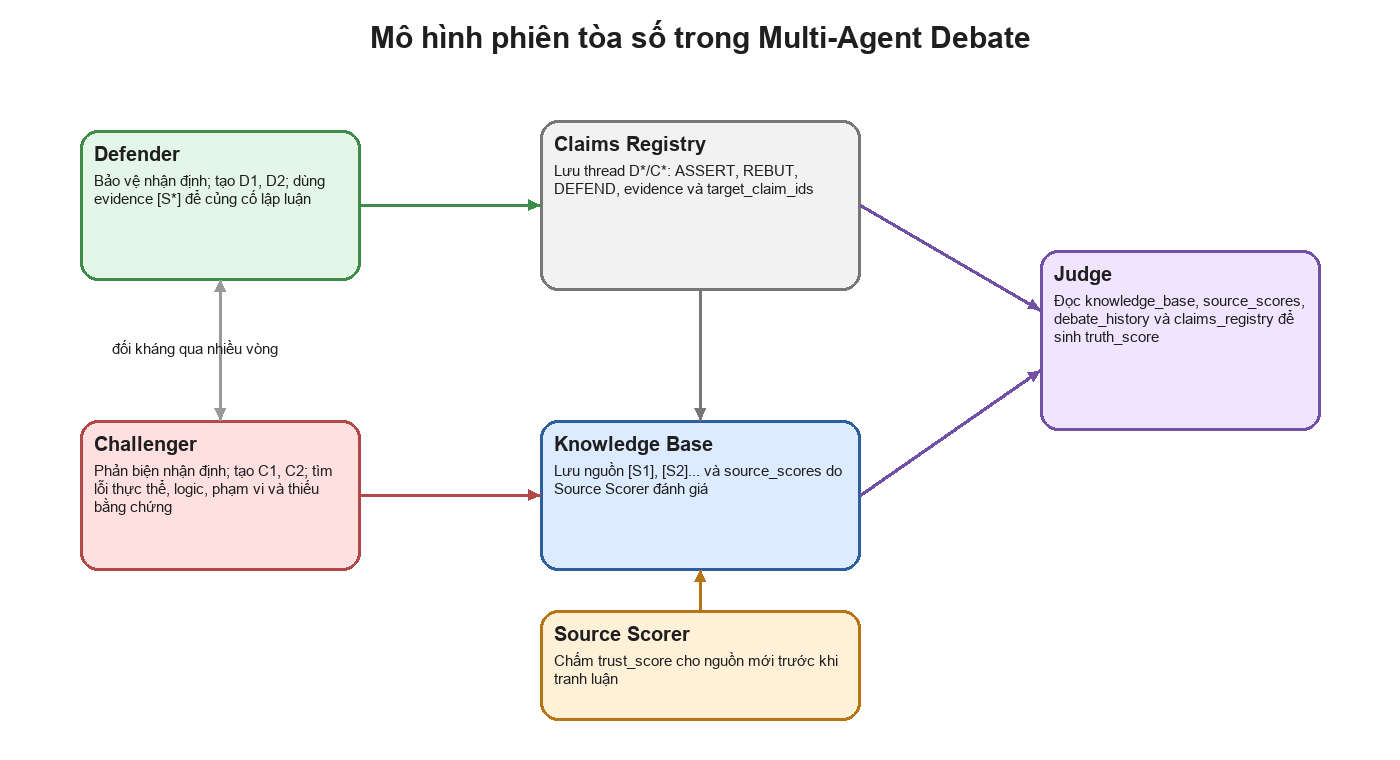
\includegraphics[width=0.9\textwidth]{figures/mad_debate_court.png}
    \caption{Mô hình phiên tòa số trong tranh biện đa tác tử}
    \label{fig:mad-debate-court}
\end{figure}
\section{LangGraph và mô hình luồng xử lý dạng trạng thái}

Một đặc điểm quan trọng của hệ thống MAD là quá trình xử lý không phải là một quy trình xử lý tuyến tính đơn giản. Trong quy trình xử lý tuyến tính, dữ liệu thường đi qua một chuỗi bước cố định và mỗi bước chỉ chạy một lần. Ngược lại, hệ thống tranh luận đa tác tử cần lặp qua nhiều vòng, trong đó kết quả của vòng trước ảnh hưởng trực tiếp tới vòng sau. Các nguồn đã tìm thấy, các truy vấn đã thực hiện, các nhận định đã được đưa ra và các phản biện trước đó đều cần được lưu lại để tiếp tục sử dụng.

Vì lý do này, đồ án sử dụng LangGraph để mô hình hóa hệ thống dưới dạng một đồ thị trạng thái. Trong mô hình này, mỗi nút đại diện cho một bước xử lý như lập kế hoạch truy vấn, tìm kiếm bằng chứng, chấm điểm nguồn, sinh lập luận của tác tử bảo vệ, sinh lập luận của tác tử phản biện, lưu kết quả vòng tranh luận và đưa ra phán quyết. Các cạnh biểu diễn thứ tự chuyển tiếp giữa các nút. Đặc biệt, đồ thị có thể chứa vòng lặp: sau khi lưu một vòng tranh luận, hệ thống kiểm tra điều kiện dừng; nếu chưa đạt số vòng tối đa, nó quay lại bước chuẩn bị vòng tiếp theo.

Cách tiếp cận dựa trên trạng thái giúp hệ thống quản lý dữ liệu trung gian một cách rõ ràng. Thay vì truyền nhiều biến rời rạc giữa các hàm, toàn bộ thông tin quan trọng được lưu trong một cấu trúc trạng thái chung. Trạng thái này bao gồm bản tin gốc, kho bằng chứng, điểm nguồn, danh sách truy vấn đã chạy, lịch sử tranh luận, bộ quản lý nhận định, số vòng hiện tại và kết quả cuối cùng. Mỗi nút chỉ đọc phần trạng thái cần thiết và trả về phần cập nhật tương ứng. Điều này giúp hệ thống dễ mở rộng hơn: nếu cần thêm một bước đánh giá mới, một nguồn tìm kiếm mới hoặc một cơ chế kiểm tra mới, có thể bổ sung nút hoặc cập nhật trạng thái mà không cần viết lại toàn bộ quy trình xử lý.

LangGraph cũng phù hợp với đặc thù của hệ thống vì nó hỗ trợ tư duy thiết kế theo luồng xử lý. Trong bài toán này, vấn đề không chỉ là gọi mô hình ngôn ngữ, mà là điều phối nhiều lần gọi mô hình, nhiều công cụ bên ngoài và nhiều trạng thái phụ thuộc lẫn nhau. Nếu không có mô hình điều phối rõ ràng, hệ thống dễ rơi vào tình trạng khó kiểm soát: tác tử không biết vòng hiện tại là vòng nào, truy vấn bị lặp, nguồn bị trùng, hoặc tác tử phán quyết không nhận đủ lịch sử. Việc biểu diễn bằng đồ thị trạng thái giúp các bước phối hợp có tính hệ thống hơn.



\section{Các công nghệ được sử dụng}

Bảng \ref{tab:technologies} trình bày các công nghệ chính được sử dụng trong đồ án.

\begin{table}[H]
\centering
\caption{Các công nghệ chính trong hệ thống}
\label{tab:technologies}
\begin{tabular}{|p{4cm}|p{4cm}|p{6cm}|}
\hline
\textbf{Thành phần} & \textbf{Công nghệ} & \textbf{Vai trò trong hệ thống} \\
\hline
Ngôn ngữ lập trình & Python & Cài đặt luồng xử lý, tác tử, xử lý dữ liệu, bộ đánh giá và giao diện trình diễn. \\
\hline
Điều phối luồng xử lý & LangGraph & Xây dựng đồ thị trạng thái có chu kỳ, phù hợp với quá trình tranh luận nhiều vòng. \\
\hline
Giao tiếp LLM & LangChain ChatOpenAI & Kết nối tới mô hình ngôn ngữ thông qua API tương thích OpenAI. \\
\hline
Nhà cung cấp mô hình & NineRouter/OpenAI-compatible API & Cho phép thay đổi mô hình nền bằng cấu hình mà không cần thay đổi kiến trúc hệ thống. \\
\hline
Tìm kiếm bằng chứng & Tavily, Wikipedia & Thu thập nguồn thông tin phục vụ lập luận và phản biện. \\
\hline
Giao diện trình diễn & Gradio & Cung cấp giao diện nhập tin tức, chọn chế độ chạy và xem diễn biến tranh luận. \\
\hline
Dữ liệu đánh giá & FEVER & Đánh giá khả năng kiểm chứng nhận định ở chế độ nhị phân SUPPORTS/REFUTES. \\
\hline
\end{tabular}
\end{table}

Python được lựa chọn vì hệ sinh thái hỗ trợ mạnh cho trí tuệ nhân tạo, xử lý dữ liệu và xây dựng ứng dụng thử nghiệm. Các thư viện như LangChain, LangGraph, Gradio, pandas và các thư viện xử lý API có thể tích hợp trực tiếp trong cùng một môi trường. Điều này giúp nhóm triển khai nhanh các thành phần khác nhau của hệ thống, từ luồng xử lý lõi đến bộ đánh giá và giao diện trình diễn.

LangGraph đóng vai trò trung tâm trong phần điều phối. Hệ thống MAD cần chạy nhiều vòng, lưu trạng thái giữa các vòng và quyết định khi nào chuyển sang phán quyết cuối. Đây là dạng bài toán phù hợp với đồ thị trạng thái hơn là một kịch bản tuần tự đơn giản. Trong hệ thống, LangGraph giúp định nghĩa các nút chức năng, kết nối giữa chúng và điều kiện dừng dựa trên số vòng tranh luận.

LangChain ChatOpenAI được sử dụng như lớp giao tiếp với mô hình ngôn ngữ. Mặc dù tên lớp gắn với OpenAI, nó có thể làm việc với các API tương thích chuẩn OpenAI, trong đó có cấu hình qua NineRouter. Lợi ích của cách làm này là hệ thống không bị khóa cứng vào một mô hình cụ thể. Khi cần thử nghiệm với Llama, Gemma, GPT-OSS hoặc Gemini, nhóm có thể thay đổi cấu hình mô hình mà vẫn giữ nguyên kiến trúc điều phối.

Tavily và Wikipedia được sử dụng cho bước tìm kiếm bằng chứng. Tavily phù hợp với nhu cầu truy xuất web vì có thể trả về các đoạn nội dung đã được trích xuất, giúp hệ thống nhanh chóng đưa nguồn vào kho bằng chứng. Wikipedia đóng vai trò nguồn tri thức có cấu trúc và tương đối ổn định, đặc biệt hữu ích trong các truy vấn về thực thể, sự kiện phổ biến hoặc bộ đánh giá có liên quan tới tri thức bách khoa. Việc có cơ chế dự phòng từ Tavily sang Wikipedia giúp hệ thống bền hơn khi một nguồn tìm kiếm không khả dụng.

Gradio được dùng để xây dựng giao diện trình diễn. Giao diện này không phải phần cốt lõi của thuật toán, nhưng giúp minh họa cách người dùng tương tác với hệ thống: nhập bản tin, chọn chế độ tìm kiếm hoặc không tìm kiếm, cấu hình số vòng tranh luận và quan sát diễn biến lập luận. Với một đồ án hệ thống, giao diện trình diễn giúp thể hiện kết quả không chỉ qua nhật ký dòng lệnh mà còn qua một quy trình tương tác dễ quan sát hơn.

FEVER được sử dụng làm bộ dữ liệu đánh giá chính vì nó phù hợp với bài toán kiểm chứng nhận định dựa trên bằng chứng. Mỗi mẫu trong FEVER gồm một nhận định và thông tin nhãn liên quan tới việc nhận định được hỗ trợ hay bị phản bác bởi bằng chứng. Trong đồ án, nhóm sử dụng thiết lập nhị phân SUPPORTS/REFUTES để so sánh trực tiếp giữa mô hình nền đơn lẻ và hệ thống MAD. Cách thiết lập này giúp đánh giá rõ liệu quy trình tranh luận đa tác tử có cải thiện khả năng phán quyết so với cách hỏi trực tiếp mô hình hay không.
% ====================================================================

% ====================================================================
\chapter{Phân tích và thiết kế hệ thống}

% GHI CHÚ: Phần này sẽ viết ở bước tiếp theo. Trọng tâm gồm tổng quan kiến trúc, 4 thành phần chính, trạng thái MAD, chế độ tìm kiếm, chế độ không tìm kiếm và cơ chế kiểm soát lỗi.

\section{Tổng quan kiến trúc hệ thống}

Hệ thống MAD được thiết kế như một quy trình kiểm chứng thông tin nhiều giai đoạn, trong đó dữ liệu đầu vào không được đưa trực tiếp vào một mô hình để lấy kết luận ngay lập tức. Thay vào đó, bản tin hoặc nhận định cần kiểm chứng được đưa vào một luồng xử lý gồm các bước: lập kế hoạch truy vấn, thu thập bằng chứng, đánh giá nguồn, tổ chức tranh luận giữa các tác tử, lưu lịch sử tranh luận và cuối cùng tổng hợp phán quyết. Cách thiết kế này phản ánh quan điểm cốt lõi của đồ án: phát hiện tin giả không chỉ là dự đoán nhãn, mà là quá trình kiểm tra có bằng chứng và có phản biện.

Ở mức tổng quát, kiến trúc hệ thống bắt đầu từ dữ liệu đầu vào của người dùng, sau đó hệ thống lập kế hoạch truy vấn, thu thập hoặc nạp bằng chứng, đánh giá nguồn, tổ chức tranh luận giữa tác tử bảo vệ và tác tử phản biện, lưu lại trạng thái của từng vòng, rồi chuyển toàn bộ thông tin cho tác tử phán quyết để sinh kết luận và giải thích cuối cùng.

\begin{figure}[H]
    \centering
    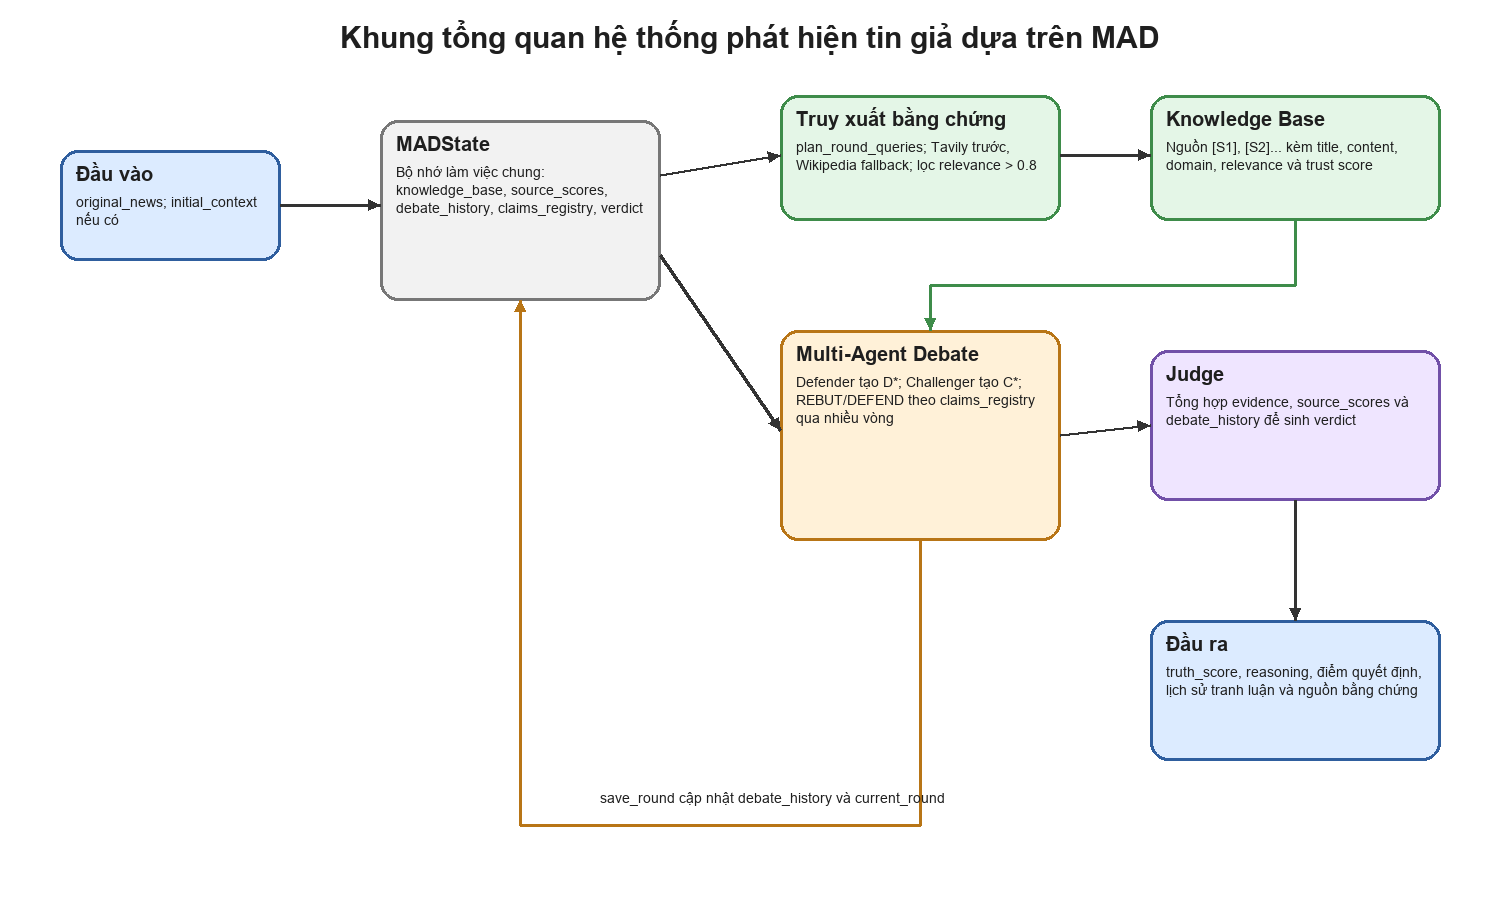
\includegraphics[width=0.95\textwidth]{figures/mad_system_overview.png}
    \caption{Khung tổng quan hệ thống phát hiện tin giả dựa trên MAD}
    \label{fig:mad-system-overview}
\end{figure}

Điểm khác biệt giữa kiến trúc này và một quy trình xử lý xử lý văn bản thông thường nằm ở việc hệ thống duy trì trạng thái xuyên suốt nhiều vòng. Trong một quy trình xử lý tuyến tính, mỗi bước thường chỉ nhận dữ liệu từ bước trước và sinh dữ liệu cho bước sau. Trong hệ thống MAD, mỗi vòng tranh luận đều có thể sử dụng lại toàn bộ thông tin đã tích lũy: nguồn bằng chứng đã tìm được, điểm tin cậy của nguồn, các truy vấn đã thực hiện, các nhận định đã được đưa ra, các phản biện trước đó và trạng thái vòng hiện tại. Điều này giúp hệ thống có khả năng phát triển lập luận theo thời gian thay vì chỉ sinh một câu trả lời độc lập.

Kiến trúc tổng thể gồm hai lớp chính. Lớp thứ nhất là lớp điều phối luồng xử lý, chịu trách nhiệm xác định nút nào được chạy, chạy theo thứ tự nào, khi nào lặp lại và khi nào dừng. Lớp này được triển khai bằng LangGraph. Lớp thứ hai là lớp tác tử và công cụ, bao gồm các thành phần thực hiện nhiệm vụ cụ thể như lập kế hoạch tìm kiếm, truy xuất bằng chứng, sinh lập luận, chấm điểm nguồn và phán quyết. Hai lớp này phối hợp thông qua một trạng thái dùng chung gọi là trạng thái MAD.

Trạng thái MAD đóng vai trò như bộ nhớ làm việc của toàn bộ hệ thống. Khi người dùng nhập một bản tin, nội dung này được lưu vào trường \texttt{original\_news}. Nếu hệ thống chạy ở chế độ không tìm kiếm, ngữ cảnh đầu vào được lưu vào \texttt{initial\_context} và sau đó được nạp thành nguồn [S1]. Trong quá trình chạy, các nguồn tìm được được thêm vào \texttt{knowledge\_base}, điểm nguồn được lưu trong \texttt{source\_scores}, lịch sử tranh luận được lưu trong \texttt{debate\_history}, còn các nhận định D1, D2, C1, C2 được quản lý trong \texttt{claims\_registry}. Kết quả cuối cùng được lưu trong \texttt{verdict}. Nhờ cách tổ chức này, mọi nút trong đồ thị đều làm việc trên cùng một bức tranh trạng thái thay vì trao đổi dữ liệu rời rạc.

Hệ thống hỗ trợ hai chế độ vận hành. Chế độ thứ nhất là \textit{chế độ tìm kiếm}, dùng cho tình huống kiểm chứng mở. Ở chế độ này, mỗi vòng tranh luận bắt đầu bằng bước lập kế hoạch truy vấn cho cả hai phía. Sau đó, hệ thống thực hiện tìm kiếm bằng chứng, chấm điểm nguồn mới, rồi mới cho tác tử bảo vệ và tác tử phản biện tranh luận. Chế độ này phù hợp khi người dùng nhập một bản tin mới mà không cung cấp sẵn tài liệu nền.

Chế độ thứ hai là \textit{chế độ không tìm kiếm}, dùng cho tình huống kiểm chứng trong phạm vi ngữ cảnh đã biết. Ở chế độ này, hệ thống không gọi công cụ tìm kiếm bên ngoài. Thay vào đó, ngữ cảnh ban đầu được xem như nguồn bằng chứng chính và được nạp vào kho bằng chứng với mã [S1]. tác tử bảo vệ và tác tử phản biện chỉ được lập luận dựa trên nguồn này và lịch sử tranh luận. Chế độ này đặc biệt phù hợp với bộ đánh giá FEVER, vì mỗi nhận định trong quá trình đánh giá có thể đi kèm bằng chứng Wikipedia đã được chuẩn bị trước. Nhờ đó, kết quả đánh giá tập trung hơn vào năng lực suy luận và tranh luận của hệ thống thay vì bị ảnh hưởng bởi chất lượng tìm kiếm web.

Một đặc điểm quan trọng khác của kiến trúc là sự tách biệt giữa bằng chứng, lập luận và phán quyết. Bằng chứng được lưu trong kho bằng chứng. Lập luận được sinh bởi tác tử bảo vệ và tác tử phản biện, sau đó lưu trong lịch sử tranh luận và bộ quản lý nhận định. Phán quyết được đưa ra bởi tác tử phán quyết ở bước cuối, dựa trên toàn bộ bằng chứng và lịch sử lập luận. Sự tách biệt này giúp hệ thống dễ kiểm tra hơn. Nếu kết quả sai, có thể phân tích lỗi thuộc về bước nào: tìm kiếm thiếu nguồn, nguồn có điểm tin cậy thấp, tác tử diễn giải sai nguồn, hay tác tử phán quyết tổng hợp chưa hợp lý.

Quy trình nhiều vòng cũng là yếu tố làm tăng độ phức tạp và giá trị của hệ thống. Ở vòng đầu, các tác tử thường đưa ra nhận định nền tảng. Ở các vòng sau, chúng không chỉ sinh thêm ý mới, mà phải phản hồi vào các nhận định cụ thể đã xuất hiện trước đó. Điều này tạo ra một chuỗi lập luận có quan hệ nhân quả: một nhận định có thể bị tấn công, được bảo vệ, tiếp tục bị phản biện hoặc bị tác tử phán quyết xem là không đủ căn cứ. Nhờ bộ quản lý nhận định, các quan hệ này không bị mất trong văn bản tự do mà được lưu thành cấu trúc có thể truy vết.

Từ góc nhìn người dùng, đầu ra của hệ thống không chỉ là một điểm số. Người dùng có thể quan sát diễn biến tranh luận, nguồn nào được trích dẫn, phía nào đưa ra lập luận thuyết phục hơn và tác tử phán quyết dựa vào đâu để kết luận. Đây là điểm quan trọng đối với một hệ thống phát hiện tin giả, vì trong nhiều trường hợp, khả năng giải thích và thuyết phục người đọc quan trọng không kém nhãn dự đoán cuối cùng.

Tóm lại, kiến trúc hệ thống MAD được xây dựng xoay quanh ba nguyên tắc: có bằng chứng, có phản biện và có truy vết. Có bằng chứng giúp hệ thống giảm phụ thuộc vào trí nhớ nội tại của LLM. Có phản biện giúp hạn chế câu trả lời một chiều. Có truy vết giúp người dùng và người phát triển phân tích được quá trình ra quyết định. Ba nguyên tắc này là nền tảng cho các thành phần chi tiết được trình bày trong các mục tiếp theo.
\section{Các thành phần chính của hệ thống}

Hệ thống MAD được xây dựng từ nhiều thành phần có vai trò khác nhau. Các thành phần này không hoạt động độc lập hoàn toàn, mà phối hợp thông qua trạng thái chung của luồng xử lý. Trong đó, tác tử bảo vệ và tác tử phản biện là hai tác tử tạo ra lõi tranh luận; Mô-đun lập kế hoạch truy vấn và tìm kiếm cung cấp bằng chứng; Bộ đánh giá nguồn đánh giá chất lượng nguồn; bộ quản lý nhận định duy trì cấu trúc lập luận; và Tác tử phán quyết tổng hợp kết quả cuối cùng. Mỗi thành phần giải quyết một phần của bài toán kiểm chứng thông tin, nhưng giá trị chính của hệ thống đến từ cách chúng được điều phối thành một quy trình thống nhất.

\subsection{Tác tử bảo vệ}

Tác tử bảo vệ là tác tử đảm nhận vai trò bảo vệ bản tin hoặc nhận định đầu vào. Trong mô hình tranh luận của hệ thống, tác tử bảo vệ đại diện cho phía cố gắng chứng minh rằng thông tin ban đầu là đúng, hợp lý hoặc ít nhất có cơ sở để được tin tưởng. Vai trò này không có nghĩa hệ thống mặc định tin bản tin là đúng, mà nhằm tạo ra một phía lập luận có chủ đích để mọi khả năng ủng hộ nhận định đều được khai thác trước khi tác tử phán quyết đưa ra kết luận.

Đầu vào của tác tử bảo vệ gồm bản tin gốc, kho bằng chứng hiện tại, điểm tin cậy của các nguồn, lịch sử tranh luận trước đó, các truy vấn đã thực hiện và danh sách mục tiêu cần phản hồi. Ở vòng đầu tiên, tác tử bảo vệ thường tập trung xây dựng các nhận định nền tảng để bảo vệ bản tin. Ở các vòng sau, tác tử bảo vệ phải quan sát các nhận định của tác tử phản biện và lựa chọn cách phản hồi: phản bác một nhận định của tác tử phản biện hoặc bảo vệ một nhận định trước đó của chính tác tử bảo vệ nếu nhận định đó bị tấn công.

Đầu ra của tác tử bảo vệ không chỉ là một đoạn văn bản tự do. Hệ thống yêu cầu lập luận được biểu diễn thành các tương tác có cấu trúc. Mỗi tương tác có loại hành động, nội dung lập luận, bằng chứng liên quan và nhận định mục tiêu nếu có. Ở vòng đầu, hành động chủ yếu là \texttt{ASSERT}, tức tạo ra một nhận định mới. Các nhận định này được gán mã D1, D2, D3,... Trong các vòng sau, Tác tử bảo vệ sử dụng \texttt{REBUT} để phản bác nhận định của tác tử phản biện hoặc \texttt{DEFEND} để bảo vệ một nhận định D* đã bị tấn công.

Việc gán mã định danh cho nhận định của tác tử bảo vệ có ý nghĩa quan trọng. Nếu tác tử bảo vệ chỉ sinh văn bản dài, hệ thống rất khó xác định câu nào là luận điểm chính, câu nào là giải thích phụ và câu nào cần được phản biện ở vòng tiếp theo. Khi mỗi nhận định được gán mã D*, các tác tử khác và tác tử phán quyết có thể tham chiếu trực tiếp đến nhận định đó. Điều này biến quá trình tranh luận từ một chuỗi văn bản phi cấu trúc thành một tập các luồng lập luận có thể theo dõi.

Tác tử bảo vệ sử dụng bằng chứng trong kho bằng chứng để củng cố lập luận. Một lập luận mạnh không chỉ nói rằng bản tin có vẻ đúng, mà phải chỉ ra nguồn nào hỗ trợ cho phần nào của nhận định. Tuy nhiên, hệ thống cũng cần kiểm soát việc sử dụng nguồn của tác tử bảo vệ. Nếu tác tử bảo vệ trích dẫn một nguồn không thực sự chứa nội dung được khẳng định, tác tử phản biện có thể phản bác và tác tử phán quyết có thể giảm trọng lượng của lập luận. Cơ chế này giúp hạn chế tình trạng tác tử sử dụng nguồn một cách hình thức.

Trong toàn bộ luồng xử lý, tác tử bảo vệ có vai trò đảm bảo rằng hệ thống không kết luận sai chỉ vì bỏ qua các bằng chứng ủng hộ. Với nhiều nhận định, đặc biệt là nhận định ngắn hoặc mơ hồ, bằng chứng hỗ trợ có thể không hiển nhiên ở lần đọc đầu. Tác tử bảo vệ buộc hệ thống phải thử xây dựng trường hợp tốt nhất cho bản tin trước khi bác bỏ nó. Đây là một nguyên tắc quan trọng trong kiểm chứng công bằng: một thông tin chỉ nên bị xem là sai sau khi các khả năng hợp lý để bảo vệ nó đã được xem xét.

\subsection{Tác tử phản biện}

Tác tử phản biện là tác tử đảm nhận vai trò phản biện. Nếu Tác tử bảo vệ cố gắng bảo vệ bản tin, Tác tử phản biện có nhiệm vụ tìm các điểm cho thấy bản tin sai, sai lệch, thiếu căn cứ hoặc bị diễn giải quá mức. Tác tử phản biện là thành phần tạo ra áp lực đối kháng chính trong hệ thống. Nhờ có tác tử phản biện, các lập luận của tác tử bảo vệ không được chấp nhận một cách dễ dàng mà phải vượt qua quá trình kiểm tra.

Đầu vào của Tác tử phản biện tương tự tác tử bảo vệ: bản tin gốc, kho bằng chứng, điểm nguồn, lịch sử tranh luận, bộ quản lý nhận định và các mục tiêu cần phản hồi. Tuy nhiên, mục tiêu sử dụng thông tin của tác tử phản biện khác với tác tử bảo vệ. Tác tử phản biện tìm kiếm các khoảng trống giữa nhận định và bằng chứng. Một nguồn có thể liên quan tới chủ đề của bản tin nhưng không trực tiếp xác nhận chi tiết quan trọng. Một nhân vật có thể có thật nhưng sự kiện gán cho nhân vật đó lại sai. Một con số có thể đúng trong phạm vi tổng quát nhưng bị áp dụng sai vào một phạm vi hẹp hơn. Đây là các dạng lỗi mà tác tử phản biện cần phát hiện.

Đầu ra của tác tử phản biện cũng được tổ chức thành các tương tác có cấu trúc. Ở vòng đầu, tác tử phản biện tạo các nhận định C1, C2, C3,... nhằm chỉ ra các lý do khiến bản tin có thể sai hoặc thiếu căn cứ. Ở các vòng sau, tác tử phản biện dùng \texttt{REBUT} để tấn công các nhận định D* của tác tử bảo vệ hoặc \texttt{DEFEND} để bảo vệ các nhận định C* của chính mình khi bị tác tử bảo vệ phản bác. Cách tổ chức này giúp tác tử phản biện không chỉ đưa ra nghi ngờ chung chung, mà phải nhắm vào các luận điểm cụ thể trong cuộc tranh luận.

Tác tử phản biện đặc biệt quan trọng trong việc phát hiện các lỗi ngữ nghĩa và lỗi suy luận. Trong nhiều trường hợp, tin giả không bịa đặt hoàn toàn mà dựa trên một phần sự thật rồi suy diễn quá mức. Ví dụ, một nguồn có thể nói rằng cà phê có liên quan tới một số lợi ích sức khỏe, nhưng bản tin lại khẳng định uống một lượng cụ thể giúp giảm một tỷ lệ rất lớn nguy cơ mắc bệnh. Nếu không có tác tử phản biện, hệ thống có thể bị thuyết phục bởi sự liên quan bề mặt giữa nguồn và nhận định. Tác tử phản biện giúp tách biệt giữa ``có liên quan'' và ``thực sự chứng minh''.

Một nhiệm vụ khác của tác tử phản biện là kiểm tra sự im lặng của nguồn. Trong kiểm chứng thông tin, việc một nguồn không đề cập tới một chi tiết quan trọng cũng có thể là dấu hiệu đáng chú ý. Nếu tác tử bảo vệ dùng một nguồn để bảo vệ nhận định nhưng nguồn đó không chứa thông tin then chốt, Tác tử phản biện có thể chỉ ra rằng bằng chứng không đủ mạnh. Đây là điểm khác với các hệ thống chỉ kiểm tra xem tài liệu có cùng chủ đề hay không. Hệ thống MAD yêu cầu nguồn phải hỗ trợ đúng nội dung được khẳng định.

Trong luồng xử lý tổng thể, Tác tử phản biện giúp giảm nguy cơ hệ thống kết luận quá dễ dãi. Nếu tác tử bảo vệ là cơ chế đảm bảo các bằng chứng ủng hộ được xem xét, thì tác tử phản biện là cơ chế đảm bảo các lỗ hổng được phơi bày. Sự cân bằng giữa hai tác tử này tạo ra nền tảng cho tác tử phán quyết đưa ra phán quyết có cơ sở hơn. Một kết luận cuối cùng đáng tin không phải vì một bên nói thuyết phục, mà vì lập luận của bên đó đứng vững hơn sau quá trình phản biện.

\subsection{Mô-đun lập kế hoạch truy vấn và tìm kiếm}

Mô-đun lập kế hoạch truy vấn và tìm kiếm là thành phần chịu trách nhiệm chuẩn bị nguồn bằng chứng cho quá trình tranh luận. Trong hệ thống MAD, tìm kiếm không được xem là một bước phụ đơn giản, mà là một phần quan trọng của chiến lược lập luận. Nếu hệ thống tìm kiếm kém, kho bằng chứng sẽ thiếu thông tin, khiến tác tử bảo vệ và tác tử phản biện phải dựa nhiều hơn vào suy đoán. Ngược lại, nếu hệ thống tìm kiếm được nguồn liên quan và đa chiều, tranh luận sẽ có nền tảng tốt hơn.

Ở mỗi vòng trong chế độ tìm kiếm, hệ thống lập kế hoạch truy vấn riêng cho từng phía. tác tử bảo vệ có thể cần các truy vấn nhằm tìm bằng chứng ủng hộ bản tin, trong khi tác tử phản biện có thể cần các truy vấn nhằm kiểm tra điểm yếu, tìm nguồn phản bác hoặc xác nhận xem chi tiết quan trọng có thật sự tồn tại hay không. Việc tách truy vấn theo phía giúp quá trình thu thập bằng chứng phản ánh đúng tính chất đối kháng của MAD. Hai phía không chỉ dùng cùng một từ khóa chung, mà có thể tiếp cận vấn đề từ các góc nhìn khác nhau.

Một yêu cầu quan trọng của lập kế hoạch truy vấn là tránh lặp lại truy vấn đã thực hiện. Hệ thống lưu các truy vấn trong \texttt{executed\_queries} để các vòng sau không tiếp tục tìm cùng một nội dung. Điều này tiết kiệm chi phí tìm kiếm, giảm lặp nguồn và khuyến khích các tác tử mở rộng hướng điều tra thay vì chỉ quay lại các bằng chứng đã có.

Sau khi có kế hoạch truy vấn, hệ thống thực hiện tìm kiếm bằng Tavily nếu API khả dụng. Tavily phù hợp cho hệ thống vì kết quả thường đi kèm phần nội dung đã được trích xuất, giúp đưa nhanh vào kho bằng chứng. Nếu Tavily không khả dụng hoặc truy vấn không trả về kết quả phù hợp, hệ thống sử dụng Wikipedia như cơ chế dự phòng. Các nguồn tìm được được lọc theo độ liên quan và được gán mã [Sx], ví dụ [S1], [S2], để sử dụng trong tranh luận.

\subsection{Bộ đánh giá nguồn}

Bộ đánh giá nguồn là thành phần đánh giá độ tin cậy của các nguồn đã được đưa vào kho bằng chứng. Trong kiểm chứng thông tin, không phải mọi bằng chứng đều có giá trị như nhau. Một nguồn từ tổ chức uy tín, bách khoa toàn thư hoặc cơ quan báo chí chính thống thường có trọng lượng cao hơn một bài viết không rõ tác giả hoặc nội dung diễn đàn. Vì vậy, hệ thống cần một bước tách biệt để đánh giá nguồn trước khi Tác tử phán quyết tổng hợp phán quyết.

Đầu vào của bộ đánh giá nguồn gồm bản tin gốc và danh sách nguồn mới chưa được chấm điểm. Với mỗi nguồn, hệ thống xem xét các thông tin như tiêu đề, miền nguồn, nội dung trích xuất và mức độ liên quan tới nhận định. Đầu ra là \texttt{source\_scores}, ánh xạ từ mã nguồn [Sx] tới điểm tin cậy trong khoảng 0.0 đến 1.0. Điểm này không tự động quyết định nhận định đúng hay sai, nhưng ảnh hưởng tới trọng lượng của lập luận dựa trên nguồn đó.

Việc tách bộ đánh giá nguồn khỏi tác tử bảo vệ và Tác tử phản biện giúp giảm xung đột vai trò. Tác tử bảo vệ có xu hướng tận dụng nguồn để bảo vệ bản tin; Tác tử phản biện có xu hướng dùng nguồn để phản bác. Nếu để mỗi bên tự đánh giá độ tin cậy của nguồn, kết quả có thể thiên lệch theo mục tiêu tranh luận. Bộ đánh giá nguồn cung cấp một lớp đánh giá trung gian, giúp tác tử phán quyết có thêm cơ sở để cân nhắc chất lượng bằng chứng.

\subsection{Bộ quản lý nhận định}

Bộ quản lý nhận định là một trong những thành phần quan trọng nhất để biến quá trình tranh luận thành một cấu trúc có thể theo dõi. Nếu không có bộ quản lý nhận định, các tác tử có thể sinh ra các đoạn văn dài qua nhiều vòng, nhưng hệ thống khó biết nhận định nào đang được bảo vệ, nhận định nào đã bị phản bác và nhận định nào còn liên quan tới kết luận cuối cùng. Bộ quản lý nhận định giải quyết vấn đề này bằng cách lưu toàn bộ nhận định dưới dạng các luồng có định danh.

Mỗi nhận định gốc của tác tử bảo vệ được gán mã D1, D2, D3,... và mỗi nhận định gốc của tác tử phản biện được gán mã C1, C2, C3,... Khi một nhận định được tạo ra, bộ quản lý lưu nội dung, vòng tranh luận, phía tạo ra, loại hành động và bằng chứng liên quan. Khi một tác tử phản biện hoặc bảo vệ nhận định đó ở vòng sau, tương tác mới được gắn vào lịch sử của cùng nhận định. Nhờ vậy, mỗi nhận định không chỉ là một câu đơn lẻ, mà là một chuỗi tương tác qua thời gian.

Cách tổ chức này buộc các tác tử phải nhắm vào mục tiêu cụ thể. Ở vòng 2 trở đi, một phản biện hợp lệ cần chỉ ra nó đang phản biện nhận định nào. Điều này giảm nguy cơ tranh luận lan man hoặc tạo thêm nhận định mới không liên quan. Đồng thời, bộ quản lý nhận định giúp tác tử phán quyết xem được toàn bộ lịch sử của một luận điểm: nó được đưa ra khi nào, đã bị ai phản bác, được bảo vệ ra sao và có bằng chứng nào đi kèm.

\subsection{Tác tử phán quyết}

Tác tử phán quyết là tác tử đưa ra phán quyết cuối cùng sau khi quá trình tranh luận kết thúc. Tác tử phán quyết không chỉ đọc bản tin gốc, mà nhận toàn bộ kho bằng chứng, điểm nguồn, lịch sử tranh luận và các nhận định đã được tạo ra. Vai trò của tác tử phán quyết là tổng hợp các bằng chứng và lập luận cạnh tranh để đưa ra một điểm chân thực cuối cùng.

Tác tử phán quyết cần đánh giá không chỉ nội dung lập luận mà cả chất lượng lập luận. Một lập luận có thể bị giảm trọng lượng nếu trích dẫn nguồn không hỗ trợ đúng nội dung, nếu lặp lại ý cũ mà không có bằng chứng mới, nếu đánh tráo khái niệm hoặc nếu không liên quan trực tiếp tới nhận định ban đầu. Ngược lại, một lập luận có nguồn rõ ràng, liên quan trực tiếp và giải quyết được phản biện của phía đối lập sẽ có trọng lượng cao hơn.

Đầu ra của tác tử phán quyết được tổ chức dưới dạng có cấu trúc. Các trường quan trọng gồm \texttt{truth\_score}, các điểm quyết định chính và phần giải thích cuối cùng. \texttt{truth\_score} biểu diễn mức độ hệ thống đánh giá bản tin là đúng. Các điểm quyết định giúp người đọc biết yếu tố nào ảnh hưởng mạnh nhất tới phán quyết. Phần giải thích cuối cùng tổng hợp lại vì sao hệ thống nghiêng về đúng, sai hoặc không chắc chắn.

Tác tử phán quyết là bước cuối cùng nhưng không phải thành phần duy nhất quyết định chất lượng hệ thống. Nếu kho bằng chứng thiếu nguồn, nếu tác tử bảo vệ hoặc Tác tử phản biện lập luận yếu, hoặc nếu bộ quản lý nhận định không tổ chức tốt lịch sử tranh luận, tác tử phán quyết sẽ có ít cơ sở để phán quyết. Vì vậy, tác tử phán quyết phụ thuộc vào toàn bộ luồng xử lý phía trước.

\begin{figure}[H]
    \centering
    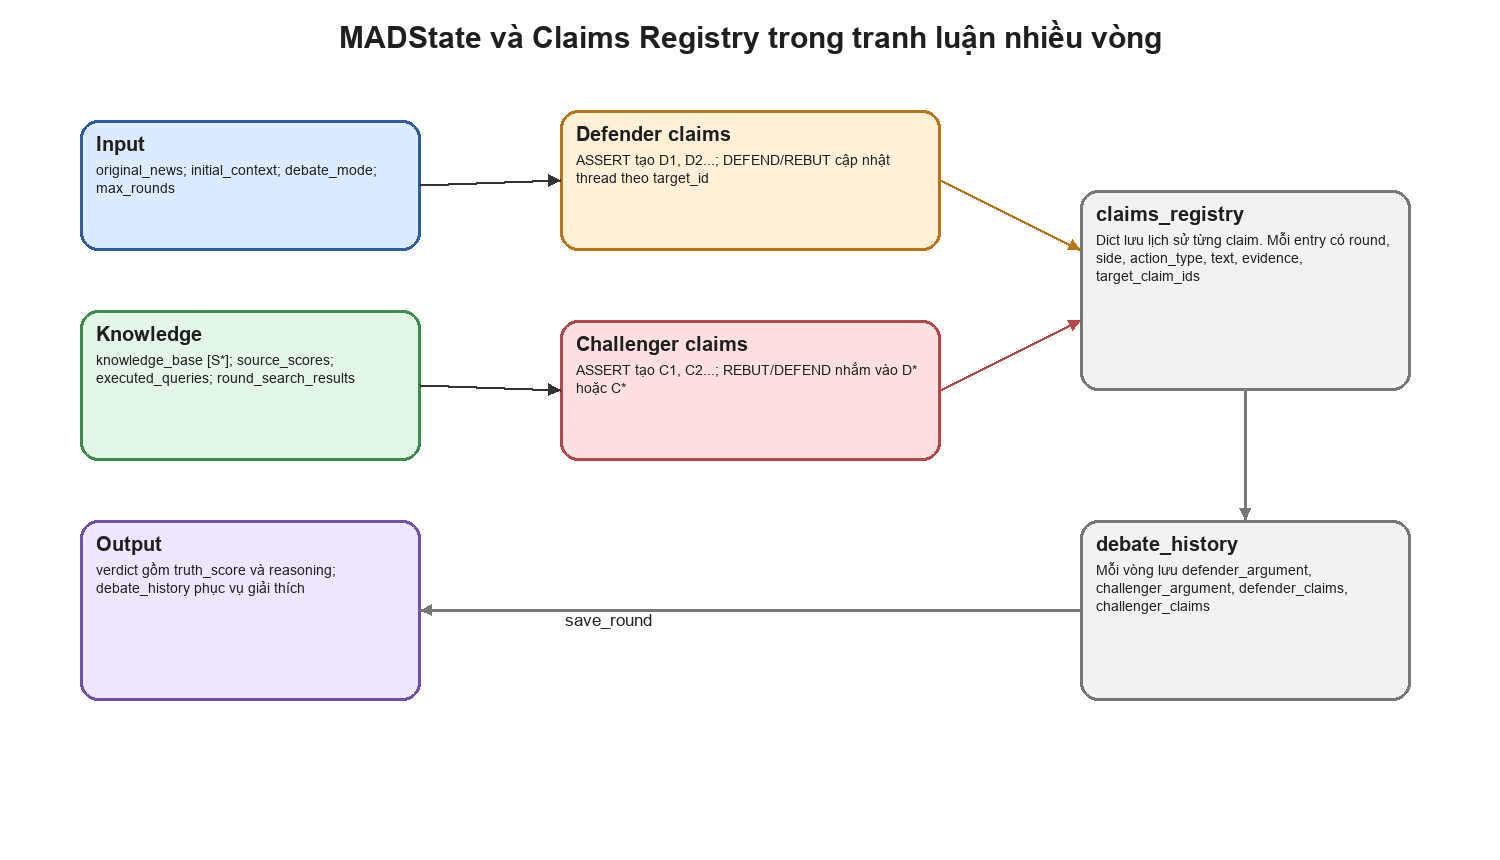
\includegraphics[width=0.95\textwidth]{figures/mad_state_claims_registry.png}
    \caption{Cách MADState liên kết kho bằng chứng, lịch sử tranh luận và claims registry}
    \label{fig:mad-state-claims}
\end{figure}
\section{Thiết kế trạng thái hệ thống}

Trạng thái MAD là cấu trúc trạng thái trung tâm của hệ thống. Toàn bộ luồng xử lý LangGraph vận hành bằng cách truyền và cập nhật trạng thái này qua các nút. Mỗi nút nhận vào trạng thái hiện tại, đọc các trường cần thiết, thực hiện nhiệm vụ của mình và trả về phần cập nhật. Cách thiết kế này giúp hệ thống nhiều vòng có thể duy trì bộ nhớ làm việc chung mà không cần truyền dữ liệu rời rạc giữa các hàm.

Bảng \ref{tab:madstate} tóm tắt các nhóm thông tin chính trong trạng thái MAD.

\begin{longtable}{|p{3.2cm}|p{4.2cm}|p{6.6cm}|}
\caption{Các nhóm trạng thái chính trong trạng thái MAD}
\label{tab:madstate}\\
\hline
\textbf{Nhóm trạng thái} & \textbf{Trường tiêu biểu} & \textbf{Ý nghĩa} \\
\hline
\endfirsthead
\hline
\textbf{Nhóm trạng thái} & \textbf{Trường tiêu biểu} & \textbf{Ý nghĩa} \\
\hline
\endhead
Đầu vào & \raggedright \small \texttt{original\_news}\\ \texttt{initial\_context} & Lưu bản tin hoặc nhận định cần kiểm chứng và ngữ cảnh ban đầu nếu có. \\
\hline
Tri thức & \raggedright \small \texttt{knowledge\_base}\\ \texttt{source\_scores} & Lưu nguồn bằng chứng và điểm tin cậy của từng nguồn. \\
\hline
Tìm kiếm & \raggedright \small \texttt{pending\_search}\\ \texttt{requests}\\ \texttt{executed\_queries}\\ \texttt{round\_search}\\ \texttt{results} & Quản lý truy vấn đang chờ, truy vấn đã chạy và kết quả tìm kiếm theo từng vòng tranh luận. \\
\hline
Tranh luận & \raggedright \small \texttt{current\_round}\\ \texttt{max\_rounds}\\ \texttt{debate\_history}\\ \texttt{claims\_registry} & Quản lý số vòng, lịch sử tranh luận và các nhận định D*/C*. \\
\hline
Đầu ra tạm thời & \raggedright \small \texttt{current\_defender}\\ \texttt{argument}\\ \texttt{current\_challenger}\\ \texttt{argument}\\ \texttt{current\_defender}\\ \texttt{claims}\\ \texttt{current\_challenger}\\ \texttt{claims} & Lưu kết quả tạm thời của tác tử bảo vệ và tác tử phản biện trong vòng hiện tại. \\
\hline
Đầu ra cuối cùng & \raggedright \small \texttt{verdict} & Lưu phán quyết cuối cùng của tác tử phán quyết. \\
\hline
\end{longtable}

Thiết kế trạng thái MAD phản ánh bản chất của hệ thống tranh luận nhiều vòng. Trong mỗi vòng, hệ thống không chỉ xử lý bản tin gốc mà còn sử dụng toàn bộ lịch sử đã tích lũy. Ví dụ, khi tác tử bảo vệ ở vòng 3 sinh lập luận, nó cần biết tác tử phản biện đã phản biện những nhận định nào ở vòng trước. Khi mô-đun tìm kiếm lập kế hoạch truy vấn, nó cần biết các truy vấn nào đã chạy để tránh lặp. Khi tác tử phán quyết phán quyết, nó cần toàn bộ lịch sử tranh luận và điểm nguồn. Nếu không có một trạng thái chung, việc phối hợp các dữ liệu này sẽ trở nên phức tạp và dễ lỗi.

Một điểm đáng chú ý là một số trường trong trạng thái MAD được cập nhật theo kiểu cộng dồn, chẳng hạn kho bằng chứng và lịch sử tranh luận. Một số trường khác chỉ giữ giá trị mới nhất, chẳng hạn lập luận hiện tại của tác tử bảo vệ hoặc tác tử phản biện. Cách phân biệt này giúp hệ thống vừa lưu được lịch sử dài hạn, vừa tránh giữ lại các giá trị tạm thời không còn cần thiết. Đây là chi tiết quan trọng trong hệ thống dựa trên LangGraph, vì mỗi nút có thể cập nhật một phần trạng thái mà không làm mất thông tin của các nút khác.

\section{Luồng xử lý ở chế độ tìm kiếm}

Chế độ tìm kiếm là chế độ vận hành đầy đủ của hệ thống, được dùng khi người dùng nhập một bản tin mới và hệ thống cần tự thu thập bằng chứng. Trong chế độ này, luồng xử lý kết hợp truy xuất thông tin, chấm điểm nguồn và tranh luận đa vòng. Luồng xử lý tổng quát của chế độ tìm kiếm gồm các pha chính: chuẩn bị vòng tranh luận, lập kế hoạch và thực hiện tìm kiếm cho từng phía, chấm điểm nguồn, sinh lập luận của tác tử bảo vệ, sinh phản biện của tác tử phản biện, lưu trạng thái vòng hiện tại, sau đó hoặc quay lại vòng tiếp theo hoặc chuyển sang phán quyết cuối cùng nếu đã đạt số vòng tối đa.

\begin{figure}[H]
    \centering
    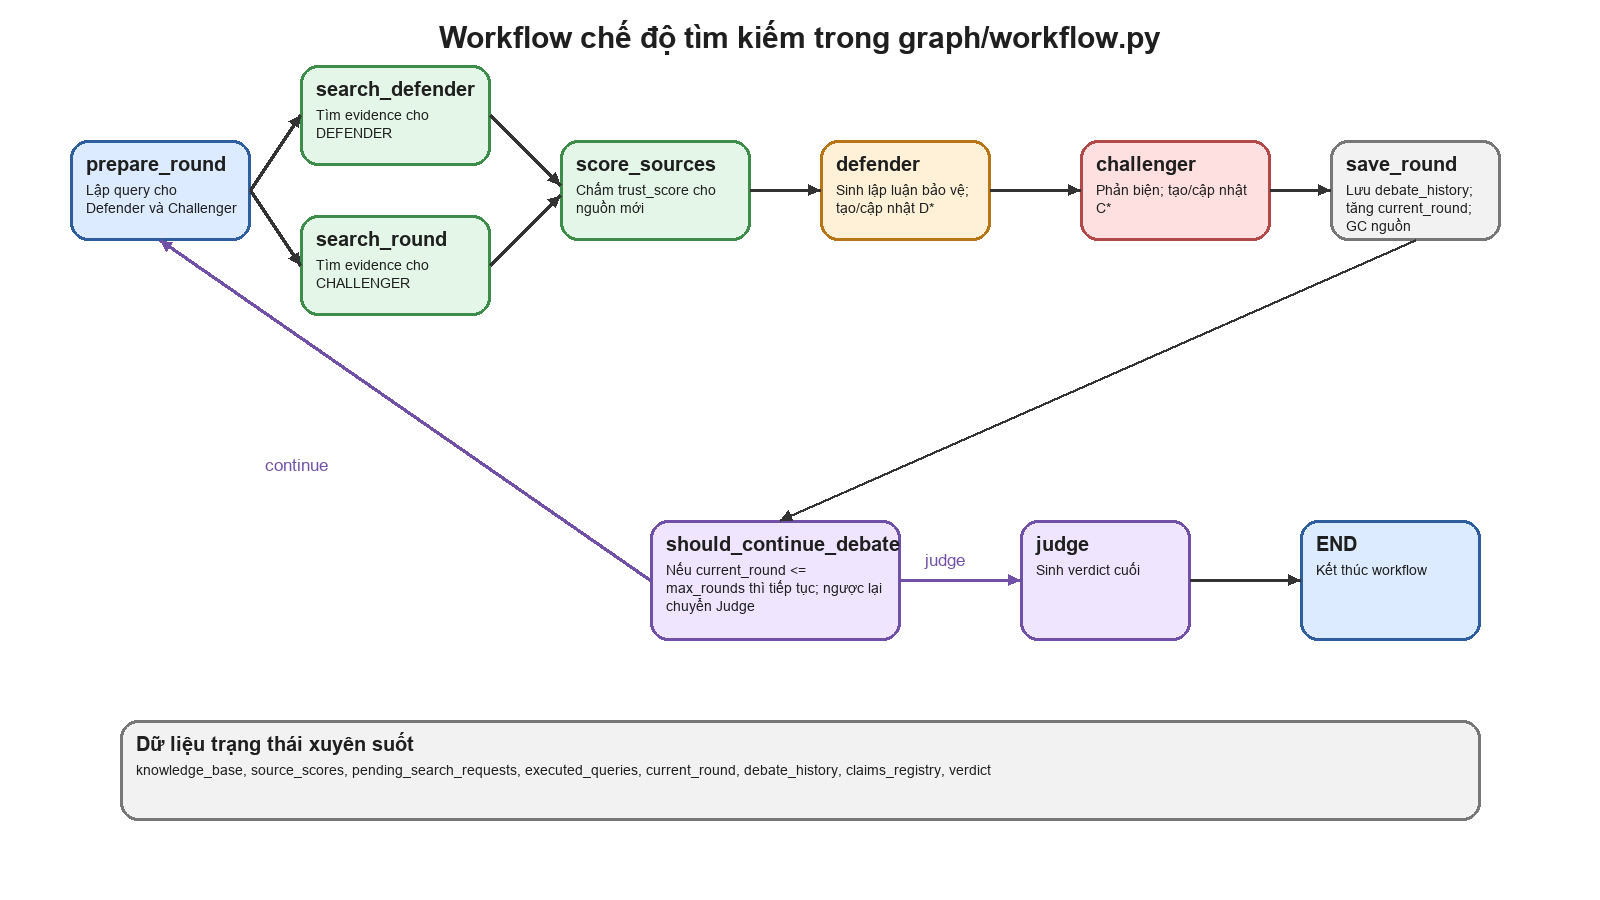
\includegraphics[width=0.95\textwidth]{figures/search_workflow.png}
    \caption{Luồng xử lý chi tiết của chế độ tìm kiếm}
    \label{fig:search-workflow-detail}
\end{figure}

Nút \texttt{prepare\_round} là điểm bắt đầu của mỗi vòng. Tại đây, hệ thống yêu cầu mỗi phía lập kế hoạch tìm kiếm dựa trên trạng thái hiện tại. Ở vòng đầu, truy vấn thường tập trung vào nội dung tổng quát của bản tin. Ở các vòng sau, truy vấn có thể nhắm vào các nhận định cụ thể đang bị tranh luận. Kết quả của nút này là danh sách yêu cầu tìm kiếm được lưu trong trường yêu cầu tìm kiếm chờ xử lý.

Sau bước chuẩn bị, hệ thống thực hiện tìm kiếm cho từng phía. Nút \texttt{search\_defender} xử lý các truy vấn phục vụ tác tử bảo vệ, còn nút \texttt{search\_round} xử lý các truy vấn phục vụ tác tử phản biện. Các kết quả phù hợp được đưa vào kho bằng chứng, đồng thời truy vấn đã chạy được ghi lại trong \texttt{executed\_queries}. Việc tách tìm kiếm theo phía giúp hệ thống phản ánh đúng mục tiêu đối kháng của hai tác tử.

Nút \texttt{score\_sources} chấm điểm các nguồn mới. Mỗi nguồn được đánh giá theo độ tin cậy và lưu vào \texttt{source\_scores}. Đây là bước quan trọng trước khi tranh luận, vì tác tử bảo vệ và tác tử phản biện có thể trích dẫn nhiều nguồn khác nhau, nhưng tác tử phán quyết cần biết nguồn nào có trọng lượng cao hơn.

Sau khi có bằng chứng, nút \texttt{defender} sinh lập luận của phía bảo vệ. Tác tử bảo vệ đọc bản tin gốc, kho bằng chứng, điểm nguồn, lịch sử tranh luận và bộ quản lý nhận định để tạo các tương tác phù hợp với vòng hiện tại. Tiếp theo, nút \texttt{challenger} sinh lập luận của phía phản biện. Tác tử phản biện cũng đọc cùng trạng thái nhưng sử dụng với mục tiêu đối lập, tập trung vào phát hiện điểm yếu hoặc thiếu căn cứ trong bản tin và trong lập luận của tác tử bảo vệ.

Nút \texttt{save\_round} lưu kết quả của vòng hiện tại vào \texttt{debate\_history}, cập nhật bộ quản lý nhận định và tăng số vòng hiện tại. Đây cũng là nơi hệ thống có thể thực hiện dọn dẹp kho bằng chứng để giảm chi phí token, ví dụ xóa nội dung chi tiết của các nguồn không được trích dẫn. Sau đó, luồng xử lý kiểm tra điều kiện dừng. Nếu số vòng hiện tại chưa vượt quá \texttt{max\_rounds}, hệ thống quay lại \texttt{prepare\_round}. Nếu đã đủ số vòng, hệ thống chuyển sang \texttt{judge}.

Nút \texttt{judge} là bước cuối cùng. Tác tử phán quyết nhận toàn bộ trạng thái đã tích lũy và sinh phán quyết. Kết quả được lưu trong \texttt{verdict}. Nhờ luồng xử lý nhiều vòng, tác tử phán quyết không chỉ nhìn thấy bản tin và nguồn bằng chứng, mà còn nhìn thấy quá trình hai phía đã kiểm tra lẫn nhau như thế nào.

\section{Luồng xử lý ở chế độ không tìm kiếm}

Chế độ không tìm kiếm là chế độ rút gọn của hệ thống, được sử dụng khi nguồn bằng chứng đã được cung cấp sẵn. Chế độ này đặc biệt phù hợp với đánh giá trên FEVER, vì mỗi nhận định có thể đi kèm đoạn bằng chứng Wikipedia. Trong chế độ này, hệ thống không gọi Tavily hoặc Wikipedia để tìm kiếm thêm, mà giới hạn lập luận trong ngữ cảnh ban đầu.

Luồng xử lý tổng quát của chế độ không tìm kiếm bắt đầu bằng việc nạp ngữ cảnh ban đầu thành nguồn [S1]. Sau đó hệ thống chuyển trực tiếp sang tác tử bảo vệ, tác tử phản biện và bước lưu vòng tranh luận. Nếu chưa đạt số vòng tối đa, hệ thống tiếp tục vòng tranh luận mới; nếu đã đủ số vòng, toàn bộ trạng thái được chuyển cho tác tử phán quyết.

Ở nút \texttt{prepare}, nếu hệ thống đang ở vòng đầu tiên, \texttt{initial\_context} được nạp vào kho bằng chứng như một nguồn đặc biệt [S1]. Nguồn này có điểm tin cậy cao vì nó được xem là ngữ cảnh chuẩn do bộ đánh giá hoặc người dùng cung cấp. Sau bước này, luồng xử lý chuyển trực tiếp sang tác tử bảo vệ và tác tử phản biện mà không qua các bước lập kế hoạch truy vấn, tìm kiếm hoặc chấm điểm nguồn.

Việc loại bỏ bước tìm kiếm giúp đánh giá tập trung hơn vào năng lực suy luận của hệ thống. Nếu chạy chế độ tìm kiếm trên bộ đánh giá, kết quả có thể bị ảnh hưởng bởi chất lượng công cụ tìm kiếm, thời điểm tìm kiếm hoặc nguồn ngoài không nằm trong dữ liệu gốc. Với chế độ không tìm kiếm, mọi mô hình đều suy luận trên cùng một ngữ cảnh, giúp việc so sánh giữa mô hình nền đơn lẻ và MAD công bằng hơn.

Tuy là chế độ rút gọn, chế độ không tìm kiếm vẫn giữ được bản chất tranh luận đa tác tử. tác tử bảo vệ vẫn phải bảo vệ nhận định dựa trên ngữ cảnh [S1], tác tử phản biện vẫn phản biện dựa trên cùng ngữ cảnh, và Tác tử phán quyết vẫn tổng hợp lịch sử tranh luận. Điều này cho phép hệ thống kiểm tra một câu hỏi quan trọng: nếu cùng được cung cấp bằng chứng, liệu cơ chế tranh luận đa tác tử có giúp đưa ra kết luận tốt hơn so với hỏi trực tiếp một LLM hay không.

\begin{figure}[H]
    \centering
    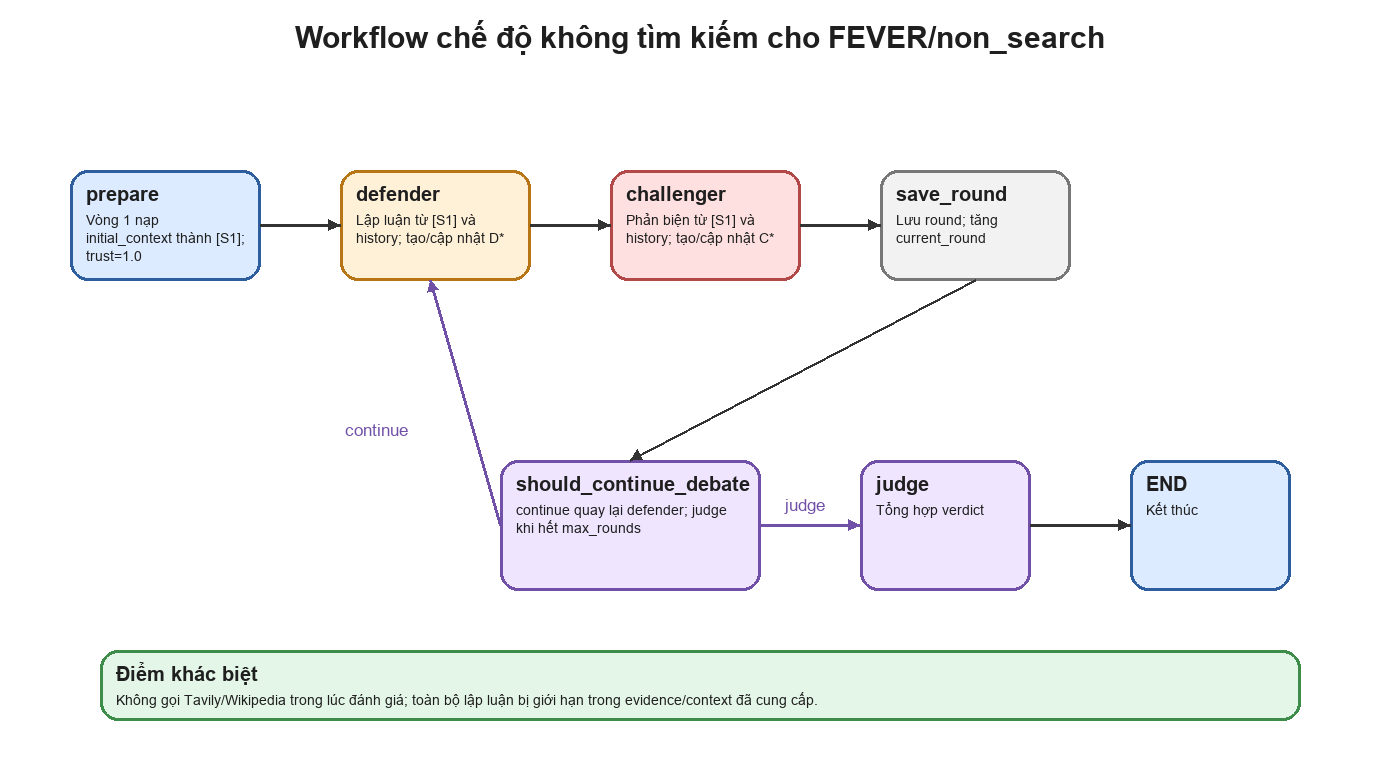
\includegraphics[width=0.9\textwidth]{figures/non_search_workflow.png}
    \caption{Luồng xử lý của chế độ không tìm kiếm dùng trong đánh giá FEVER}
    \label{fig:non-search-workflow}
\end{figure}

\section{Cơ chế kiểm soát lỗi và tối ưu tài nguyên}

Hệ thống MAD cần nhiều lần gọi mô hình ngôn ngữ và công cụ tìm kiếm, vì vậy cơ chế kiểm soát lỗi và tối ưu tài nguyên là cần thiết. Nếu không có các cơ chế này, hệ thống dễ gặp lỗi giới hạn tần suất gọi, đầu ra không đúng định dạng, ngữ cảnh quá dài hoặc kho bằng chứng chứa quá nhiều nguồn không được sử dụng.

Cơ chế thứ nhất là giới hạn tần suất gọi và thử lại. Khi gọi LLM qua API, hệ thống có thể gặp giới hạn số request theo phút hoặc lỗi quota tạm thời. Mô-đun giới hạn tần suất gọi chủ động giãn cách các lần gọi và tự động thử lại khi gặp lỗi như HTTP 429 hoặc thông báo quota. Điều này giúp quá trình bộ đánh giá dài không bị dừng ngay khi gặp lỗi tạm thời.

Cơ chế thứ hai là dự phòng trong tìm kiếm. Tavily được ưu tiên trong chế độ tìm kiếm, nhưng nếu không có khóa API hoặc gặp lỗi, hệ thống có thể chuyển sang Wikipedia. Cách này làm tăng độ bền của hệ thống, đặc biệt trong môi trường thử nghiệm nơi không phải lúc nào mọi dịch vụ bên ngoài cũng ổn định.

Cơ chế thứ ba là phân tích cú pháp nhiều tầng cho kết quả tác tử phán quyết. Vì LLM đôi khi không trả về JSON hoàn hảo, hệ thống cần cố gắng trích xuất kết quả từ nhiều dạng đầu ra khác nhau, chẳng hạn JSON thuần, JSON trong khối mã hoặc văn bản có chứa trường \texttt{truth\_score}. Cơ chế này không thay thế yêu cầu đầu ra có cấu trúc, nhưng giúp hệ thống bền hơn khi làm việc với nhiều mô hình có khả năng tuân thủ định dạng khác nhau.

Cơ chế thứ tư là dọn dẹp bộ nhớ trong kho bằng chứng. Sau mỗi vòng, hệ thống có thể xóa nội dung chi tiết của các nguồn không được trích dẫn để giảm độ dài ngữ cảnh. Việc này đặc biệt quan trọng vì tranh luận nhiều vòng có thể làm chỉ dẫn ngày càng dài. Tuy nhiên, hệ thống cần giữ lại các nguồn quan trọng, đặc biệt là nguồn ngữ cảnh ban đầu [S1] trong chế độ không tìm kiếm.

Nhìn chung, các cơ chế trên giúp hệ thống không chỉ hoạt động đúng về mặt thuật toán mà còn có khả năng vận hành thực tế hơn. Một hệ thống đa tác tử nếu không kiểm soát lỗi và tài nguyên sẽ rất khó đánh giá ổn định, vì số lần gọi mô hình nhiều hơn đáng kể so với mô hình nền đơn lẻ.
\chapter{Cài đặt và triển khai}

\section{Cấu trúc thư mục dự án}

Mã nguồn của hệ thống được tổ chức theo hướng tách biệt giữa phần điều phối luồng xử lý, phần tác tử, phần chỉ dẫn, phần cấu hình, phần tiện ích và phần thực nghiệm. Cách tổ chức này giúp mỗi nhóm chức năng có trách nhiệm rõ ràng, đồng thời thuận tiện cho việc mở rộng hệ thống trong tương lai. Về tổng thể, dự án được chia thành các nhóm thư mục chính. Thư mục \texttt{agents/} chứa các tác tử và thành phần xử lý lập luận; \texttt{graph/} chứa định nghĩa trạng thái và luồng xử lý; \texttt{prompts/} chứa các mẫu chỉ dẫn; \texttt{config/} chứa cấu hình; \texttt{utils/} chứa tiện ích vận hành; \texttt{scripts/} chứa các kịch bản chuẩn bị dữ liệu và đánh giá; \texttt{data/} lưu dữ liệu thô, dữ liệu đã xử lý và kết quả thực nghiệm. Các file \texttt{main.py}, \texttt{app.py} và \texttt{requirements.txt} lần lượt phục vụ khởi chạy hệ thống, giao diện trình diễn và quản lý phụ thuộc.

Thư mục \texttt{agents/} chứa các thành phần sinh lập luận, tìm kiếm, đánh giá nguồn và phán quyết. Đây là nơi hiện thực hóa phần lớn logic hành vi của hệ thống. \texttt{defender.py} và \texttt{challenger.py} lần lượt triển khai hai tác tử tranh luận chính. \texttt{search\_agent.py} phụ trách lập kế hoạch truy vấn và tìm kiếm bằng chứng. \texttt{evaluator.py} chứa các hàm xử lý đánh giá nguồn, chuẩn hóa JSON và định dạng kho bằng chứng. \texttt{judge.py} triển khai bước phán quyết cuối cùng.

Thư mục \texttt{graph/} là lõi điều phối của hệ thống. Tệp \texttt{state.py} định nghĩa trạng thái MAD và các reducer dùng để cập nhật trạng thái qua nhiều nút. Tệp \texttt{workflow.py} định nghĩa hai luồng xử lý chính: luồng xử lý có tìm kiếm và luồng xử lý không tìm kiếm. Việc tách luồng xử lý khỏi tác tử giúp hệ thống phân biệt rõ giữa logic điều phối và logic xử lý của từng tác tử.

Thư mục \texttt{prompts/} chứa các template điều khiển hành vi của mô hình ngôn ngữ. Trong báo cáo này, chỉ dẫn không được trình bày theo từng chi tiết nhỏ, nhưng về mặt triển khai, đây là lớp định nghĩa vai trò, định dạng đầu ra và các ràng buộc hành vi ở mức hệ thống. Thư mục \texttt{config/} chứa cấu hình mô hình và tham số tranh luận. Thư mục \texttt{utils/} chứa các tiện ích vận hành như giới hạn tần suất gọi và thử lại.

Thư mục \texttt{scripts/} phục vụ chuẩn bị dữ liệu và thực nghiệm. Các kịch bản \texttt{prepare\_*} chuyển dữ liệu thô thành dạng nhận định có thể đưa vào hệ thống. Các kịch bản \texttt{test\_*} chạy đánh giá, so sánh mô hình nền đơn lẻ và MAD, đồng thời lưu nhật ký. Thư mục \texttt{data/} được chia thành dữ liệu thô, dữ liệu đã xử lý và kết quả thực nghiệm. Hai file \texttt{main.py} và \texttt{app.py} lần lượt đóng vai trò điểm khởi chạy cho chạy hệ thống bằng mã nguồn và giao diện trình diễn.

\section{Cấu hình môi trường}

Hệ thống được triển khai bằng Python và sử dụng các thư viện được liệt kê trong \texttt{requirements.txt}. Các nhóm phụ thuộc chính gồm LangGraph, LangChain, Tavily, Wikipedia, Gradio, pandas và python-dotenv. Việc gom cấu hình phụ thuộc vào một tệp requirements giúp môi trường chạy có thể được tái tạo trên máy khác, đồng thời thuận tiện cho quá trình báo cáo và kiểm thử.

Các thông tin nhạy cảm như khóa API không được hard-code trong mã nguồn. Hệ thống sử dụng file môi trường \texttt{.env} để cấu hình khóa truy cập và endpoint. Các biến quan trọng gồm:

\begin{itemize}
    \item \texttt{NINEROUTER\_API\_KEY}: khóa API dùng để gọi mô hình ngôn ngữ.
    \item \texttt{NINEROUTER\_BASE\_URL}: endpoint API tương thích OpenAI.
    \item \texttt{NINEROUTER\_MODEL}: tên mô hình được sử dụng cho hệ thống.
    \item \texttt{TAVILY\_API\_KEY}: khóa API cho công cụ tìm kiếm Tavily, nếu chạy chế độ tìm kiếm.
\end{itemize}

Việc cấu hình mô hình thông qua biến môi trường giúp hệ thống linh hoạt khi thử nghiệm nhiều mô hình khác nhau. Trong phần thực nghiệm, nhóm có thể thay đổi mô hình nền để so sánh hiệu quả giữa mô hình nền đơn lẻ và MAD mà không cần thay đổi logic luồng xử lý. Đây là một điểm quan trọng vì mục tiêu của đồ án không phải tối ưu riêng cho một mô hình, mà đánh giá xem cơ chế tranh luận đa tác tử có tạo ra cải thiện ổn định trên nhiều mô hình hay không.

\section{Điểm khởi chạy và quy trình chạy hệ thống}

Tệp \texttt{main.py} là điểm khởi chạy chính cho việc chạy hệ thống ở mức mã nguồn. Hàm \texttt{get\_llm()} đọc cấu hình môi trường và khởi tạo đối tượng mô hình ngôn ngữ thông qua \texttt{ChatOpenAI}. Việc khởi tạo này được đặt riêng để các kịch bản thực nghiệm có thể dùng lại cùng một cách tạo mô hình, đảm bảo quá trình so sánh mô hình nền đơn lẻ và MAD sử dụng cùng cấu hình.

Hàm quan trọng nhất trong \texttt{main.py} là \texttt{run\_mad()}. Hàm này nhận vào bản tin cần kiểm chứng, ngữ cảnh ban đầu nếu có, chế độ tranh luận và tùy chọn định dạng đầu ra của tác tử phán quyết. Nếu \texttt{debate\_mode} là \texttt{search}, hệ thống xây dựng luồng xử lý có tìm kiếm. Nếu \texttt{debate\_mode} là \texttt{non\_search}, hệ thống xây dựng luồng xử lý không tìm kiếm. Sau đó, hàm tạo trạng thái ban đầu bằng \texttt{build\_initial\_state()} và gọi luồng xử lý để lấy trạng thái cuối.

Về mặt sử dụng, chế độ tìm kiếm phù hợp khi người dùng muốn kiểm chứng một bản tin mới và cho phép hệ thống tự tìm bằng chứng bên ngoài. Chế độ không tìm kiếm phù hợp khi nguồn bằng chứng đã được cung cấp sẵn, ví dụ trong bộ đánh giá FEVER. Cùng một hàm \texttt{run\_mad()} có thể phục vụ cả hai chế độ, nhờ đó logic thực nghiệm và logic trình diễn không bị tách rời hoàn toàn.

Kết quả trả về của \texttt{run\_mad()} là trạng thái cuối, trong đó quan trọng nhất là \texttt{verdict}. Tuy nhiên, trạng thái cuối cũng chứa nhiều thông tin phục vụ phân tích như kho bằng chứng, lịch sử tranh luận và các nhận định đã được sinh ra. Đây là điểm khác biệt so với hàm dự đoán thông thường chỉ trả về một nhãn. Với hệ thống MAD, quá trình chạy tạo ra cả một dấu vết kiểm chứng, giúp người phát triển phân tích vì sao hệ thống đúng hoặc sai.

\section{Triển khai luồng xử lý LangGraph}

Phần luồng xử lý được triển khai trong tệp \texttt{graph/workflow.py}. Hệ thống có hai hàm xây dựng đồ thị chính. Hàm \texttt{build\_workflow()} dùng cho chế độ tìm kiếm. Hàm xây dựng workflow không tìm kiếm dùng cho chế độ không tìm kiếm. Cả hai luồng xử lý đều dựa trên cùng trạng thái MAD, nhưng khác nhau ở cách chuẩn bị bằng chứng trước khi tranh luận.

Trong chế độ tìm kiếm, đồ thị bắt đầu từ nút \texttt{prepare\_round}, sau đó chuyển sang các nút tìm kiếm, chấm điểm nguồn, tranh luận và lưu vòng. Sau mỗi vòng, hàm điều kiện kiểm tra \texttt{current\_round} so với \texttt{max\_rounds}. Nếu chưa đủ số vòng, đồ thị quay lại bước chuẩn bị vòng mới. Nếu đã đủ, đồ thị chuyển sang tác tử phán quyết. Cách triển khai này cho phép hệ thống mở rộng tự nhiên theo số vòng tranh luận mà người dùng cấu hình.

Trong chế độ không tìm kiếm, đồ thị được rút gọn. Nút chuẩn bị chỉ cần nạp \texttt{initial\_context} thành nguồn [S1] ở vòng đầu. Sau đó đồ thị đi thẳng vào tác tử bảo vệ, tác tử phản biện, lưu vòng và tác tử phán quyết. Mặc dù ít nút hơn, luồng xử lý này vẫn dùng cùng cơ chế lịch sử tranh luận và bộ quản lý nhận định, giúp kết quả đánh giá trên bộ đánh giá giữ được bản chất tranh biện đa tác tử.

Việc triển khai bằng LangGraph giúp mã nguồn phản ánh trực tiếp thiết kế đã trình bày ở Chương 3. Mỗi nút trong đồ thị tương ứng với một chức năng rõ ràng. Điều này làm cho hệ thống dễ gỡ lỗi hơn: nếu kho bằng chứng rỗng, có thể kiểm tra nút tìm kiếm; nếu lập luận không được lưu, kiểm tra nút lưu vòng; nếu phán quyết thiếu trường, kiểm tra tác tử phán quyết. Cách tách nút như vậy cũng giúp báo cáo và mã nguồn có sự tương ứng rõ ràng.

\section{Triển khai các tác tử}

Các tác tử chính được triển khai trong thư mục \texttt{agents/}. tác tử bảo vệ và tác tử phản biện có cấu trúc xử lý tương tự nhau nhưng mục tiêu đối lập. Mỗi tác tử đọc trạng thái hiện tại, xây dựng đầu vào cho mô hình ngôn ngữ, nhận kết quả có cấu trúc và chuyển kết quả đó thành các nhận định được lưu vào registry. Việc hai tác tử có cấu trúc tương tự giúp hệ thống dễ bảo trì, đồng thời đảm bảo tính cân bằng trong tranh luận.

\texttt{search\_agent.py} triển khai hai nhóm chức năng: lập kế hoạch truy vấn và thực thi tìm kiếm. Phần lập kế hoạch sử dụng trạng thái hiện tại để tạo truy vấn phù hợp với từng phía. Phần thực thi tìm kiếm gọi Tavily hoặc Wikipedia, lọc kết quả, gán mã nguồn và thêm nguồn vào kho bằng chứng. Đây là cầu nối giữa thế giới bên ngoài và quá trình lập luận nội bộ của hệ thống.

\texttt{evaluator.py} chứa các tiện ích liên quan tới đánh giá nguồn và xử lý dữ liệu trung gian. Trong đó, chức năng chấm điểm nguồn giúp tạo \texttt{source\_scores}, còn các hàm định dạng kho bằng chứng giúp đưa nguồn vào chỉ dẫn theo dạng dễ đọc cho mô hình. File này cũng chứa logic phân tích cú pháp JSON bền hơn, phục vụ việc làm việc với đầu ra không hoàn toàn ổn định của LLM.

\texttt{judge.py} triển khai phán quyết cuối cùng. Tác tử phán quyết nhận toàn bộ lịch sử tranh luận và kho bằng chứng đã được định dạng, sau đó yêu cầu mô hình sinh kết quả theo cấu trúc mong muốn. Phần phân tích cú pháp kết quả của tác tử phán quyết được thiết kế nhiều tầng để giảm nguy cơ lỗi khi mô hình trả về JSON không hoàn hảo. Trong bối cảnh bộ đánh giá, đây là chi tiết quan trọng vì một lỗi định dạng có thể làm hỏng kết quả của cả một mẫu kiểm thử.

\section{Đầu ra có cấu trúc và thiết kế chỉ dẫn ở mức hệ thống}

Trong hệ thống MAD, chỉ dẫn không chỉ dùng để hỏi đáp thông thường mà đóng vai trò như cơ chế điều khiển hành vi của tác tử. Tuy nhiên, thay vì phụ thuộc vào các chỉ dẫn dài một cách khó kiểm soát, hệ thống thiết kế chỉ dẫn theo hướng có vai trò, pha xử lý và định dạng đầu ra rõ ràng. Báo cáo không đi sâu vào từng câu lệnh chỉ dẫn, mà tập trung vào các nguyên tắc thiết kế ở mức hệ thống.

Đối với tác tử bảo vệ và tác tử phản biện, chỉ dẫn được tổ chức theo hai pha chính. Pha thứ nhất là lập kế hoạch truy vấn, trong đó tác tử phân tích trạng thái hiện tại và đề xuất hướng tìm kiếm bằng chứng. Pha thứ hai là tranh luận, trong đó tác tử tạo lập luận dựa trên kho bằng chứng, lịch sử tranh luận và các mục tiêu cần phản hồi. Việc chia pha giúp hệ thống tách riêng hành động điều tra và hành động tranh luận.

Một yêu cầu quan trọng là đầu ra của tác tử phải có cấu trúc. Thay vì sinh văn bản tự do, tác tử cần trả về danh sách interaction với loại hành động, nội dung, bằng chứng và mục tiêu. Điều này cho phép hệ thống chuyển đầu ra của LLM thành dữ liệu có thể lưu trong bộ quản lý nhận định. Nếu không có đầu ra có cấu trúc, các bước sau như phản biện nhận định cụ thể, hiển thị lịch sử tranh luận hoặc tác tử phán quyết tổng hợp sẽ khó thực hiện ổn định.

tác tử phán quyết cũng sử dụng đầu ra chỉ dẫn riêng. Trong trình diễn thông thường, tác tử phán quyết có thể trả về điểm chân thực theo nhiều mức để phản ánh sắc thái đúng/sai. Trong bộ đánh giá nhị phân như FEVER, chỉ dẫn có thể được điều chỉnh để ép kết quả về 0.0 hoặc 1.0. Cách tách phần chỉ dẫn nền và phần chỉ dẫn đầu ra giúp cùng một tác tử phán quyết có thể phục vụ nhiều kịch bản đánh giá khác nhau.

\section{Giao diện trình diễn và nhật ký thực nghiệm}

Bên cạnh điểm khởi chạy dòng lệnh, dự án có giao diện trình diễn bằng Gradio trong \texttt{app.py}. Giao diện cho phép người dùng nhập bản tin, chọn chế độ tìm kiếm hoặc chế độ không tìm kiếm, cung cấp ngữ cảnh nếu cần và cấu hình số vòng tranh luận. Kết quả được hiển thị theo nhiều vùng: trạng thái hệ thống, nguồn dữ liệu, diễn biến tranh luận và phán quyết cuối cùng.

Vai trò của giao diện trình diễn là giúp quan sát hệ thống như một quy trình tương tác. Thay vì chỉ nhìn thấy kết quả cuối trong cửa sổ lệnh, người dùng có thể theo dõi các nhận định được sinh ra, nguồn nào được dùng và tác tử phán quyết kết luận ra sao. Điều này phù hợp với mục tiêu giải thích của đồ án. Tuy nhiên, giao diện trình diễn được xem là lớp trình bày bên ngoài; lõi hệ thống vẫn nằm ở luồng xử lý và các tác tử.

Đối với thực nghiệm, hệ thống lưu nhật ký chi tiết trong thư mục \texttt{data/results/}. Mỗi mẫu bộ đánh giá có thể được lưu kèm nhận định, nhãn đúng, kết quả mô hình nền đơn lẻ, kết quả MAD, phán quyết, lịch sử tranh luận và thời gian chạy. Nhật ký này rất quan trọng cho phân tích lỗi. Khi một mẫu bị dự đoán sai, nhóm có thể đọc lại toàn bộ tranh luận để xác định lỗi đến từ nguồn bằng chứng, lập luận của tác tử hay phán quyết của tác tử phán quyết.
\chapter{Thực nghiệm và phương pháp đánh giá}

\section{Mục tiêu thực nghiệm}

Thực nghiệm của đồ án được thiết kế nhằm đánh giá xem cơ chế tranh biện đa tác tử có mang lại lợi ích thực tế so với cách sử dụng một mô hình ngôn ngữ đơn lẻ hay không. Vì hệ thống MAD phức tạp hơn mô hình nền đơn lẻ, tiêu tốn nhiều lời gọi mô hình hơn và có nhiều bước trung gian hơn, việc đánh giá cần trả lời rõ câu hỏi: sự phức tạp bổ sung đó có tạo ra cải thiện về chất lượng phán quyết và khả năng giải thích hay không.

Mục tiêu thứ nhất là so sánh độ chính xác giữa mô hình nền đơn lẻ và hệ thống MAD. Mô hình nền đơn lẻ được hiểu là cùng một mô hình nền được hỏi trực tiếp về nhận định cần kiểm chứng. Hệ thống MAD sử dụng chính mô hình đó nhưng đặt trong luồng xử lý nhiều tác tử, có tranh luận, có ngữ cảnh và có tác tử phán quyết. Nếu MAD đạt kết quả tốt hơn, điều này cho thấy cải thiện đến từ quy trình điều phối và cơ chế tranh luận, không chỉ đến từ việc dùng một mô hình mạnh hơn.

Mục tiêu thứ hai là đánh giá khả năng giảm phán đoán thiếu căn cứ. Trong kiểm chứng thông tin, một hệ thống có thể đạt độ chính xác cao trên một số mẫu nhưng vẫn nguy hiểm nếu thường xuyên suy đoán khi bằng chứng không đủ. MAD được kỳ vọng thận trọng hơn vì các lập luận phải đối mặt với phản biện và tác tử phán quyết có thể xem xét liệu nguồn có thực sự hỗ trợ nhận định hay không.

Mục tiêu thứ ba là đánh giá khả năng giải thích. mô hình nền đơn lẻ có thể đưa ra một đoạn reasoning, nhưng reasoning đó không nhất thiết phản ánh một quá trình kiểm chứng có cấu trúc. Trong khi đó, MAD tạo ra lịch sử tranh luận, danh sách nguồn và các điểm quyết định. Vì vậy, ngoài các chỉ số định lượng, nhật ký thực nghiệm cũng được dùng để phân tích các trường hợp thành công và thất bại.

\section{Bộ dữ liệu FEVER}

FEVER là một bộ dữ liệu phổ biến cho bài toán kiểm chứng nhận định dựa trên bằng chứng \cite{thorne2018fever}. Mỗi mẫu trong FEVER gồm một nhận định và nhãn cho biết nhận định đó được hỗ trợ hay bị phản bác bởi các bằng chứng từ Wikipedia. Điều này phù hợp với mục tiêu của đồ án vì hệ thống MAD cần được đánh giá trên khả năng suy luận từ bằng chứng, không chỉ dựa vào phong cách ngôn ngữ của bản tin.

Trong phạm vi thực nghiệm chính, nhóm sử dụng hai nhãn SUPPORTS và REFUTES. Các mẫu SUPPORTS được quy đổi thành nhãn 1.0, biểu diễn nhận định đúng theo bằng chứng. Các mẫu REFUTES được quy đổi thành nhãn 0.0, biểu diễn nhận định sai theo bằng chứng. Thiết lập này tạo thành bài toán nhị phân, giúp việc so sánh giữa mô hình nền đơn lẻ và MAD rõ ràng hơn.

Một điểm quan trọng của FEVER là nhận định thường ngắn nhưng đòi hỏi kiểm tra chi tiết. Một nhận định có thể phụ thuộc vào thực thể, quan hệ, vai trò, thời điểm hoặc phạm vi của một phát biểu. Vì vậy, FEVER phù hợp để kiểm tra khả năng suy luận nghiêm ngặt của hệ thống. Những lỗi như nhầm tập con với tập tổng, nhầm vai trò diễn viên, nhầm khái niệm hoặc suy diễn quá mức từ nguồn đều có thể xuất hiện trong quá trình đánh giá.

Trong thí nghiệm, dữ liệu được lấy mẫu cân bằng giữa hai nhãn. Cách lấy mẫu cân bằng giúp độ chính xác không bị lệch bởi tỷ lệ nhãn trong tập dữ liệu. Ví dụ, với 40 mẫu, hệ thống lấy 20 mẫu SUPPORTS và 20 mẫu REFUTES. Điều này giúp các chỉ số độ chính xác dương, độ bao phủ và F1-score có ý nghĩa hơn khi so sánh giữa mô hình nền đơn lẻ và MAD.

\section{Quy trình chuẩn bị dữ liệu}

Quy trình chuẩn bị dữ liệu FEVER được triển khai trong kịch bản \texttt{scripts/prepare\_fever.py}. Kịch bản này đọc dữ liệu thô từ tệp \texttt{FEVER.jsonl}, lọc các mẫu có nhãn SUPPORTS hoặc REFUTES và chỉ giữ các mẫu có thể kiểm chứng. Sau đó, kịch bản lấy danh sách trang Wikipedia liên quan từ bằng chứng của FEVER và truy xuất nội dung tóm tắt tương ứng.

Với mỗi mẫu hợp lệ, kịch bản tạo ra một bản ghi gồm mã định danh, nhận định, nhãn nhị phân, nhãn gốc và \texttt{initial\_context}. Trường \texttt{initial\_context} là phần bằng chứng được lấy từ Wikipedia, dùng làm nguồn đầu vào cho chế độ không tìm kiếm. Việc chuẩn bị sẵn ngữ cảnh giúp hệ thống đánh giá trong môi trường kiểm soát: mọi mẫu đều có nguồn bằng chứng được cung cấp trước, và MAD không cần tự tìm kiếm web trong lúc bộ đánh giá.

Dữ liệu sau xử lý được lưu vào tệp dữ liệu FEVER nhị phân đã xử lý. Đây là đầu vào chính cho kịch bản đánh giá. Cách tách bước chuẩn bị dữ liệu khỏi bước chạy thực nghiệm giúp quá trình bộ đánh giá ổn định hơn. Nếu mỗi lần đánh giá đều truy xuất lại Wikipedia, kết quả có thể bị ảnh hưởng bởi lỗi mạng hoặc thay đổi nội dung nguồn. Khi dữ liệu đã được xử lý trước, các lần chạy sau tập trung vào năng lực của mô hình và luồng xử lý.

\begin{figure}[H]
    \centering
    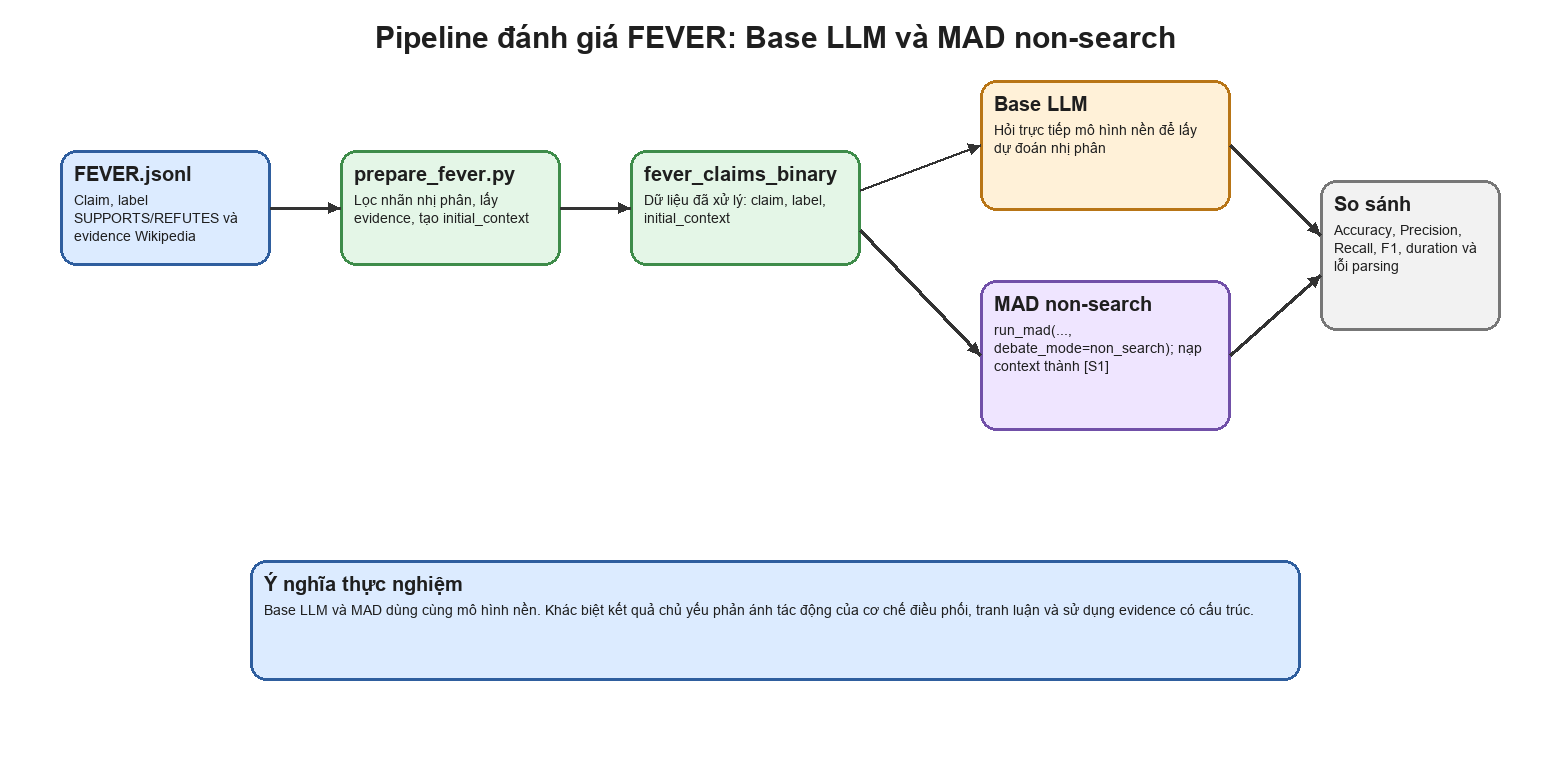
\includegraphics[width=0.95\textwidth]{figures/fever_evaluation_pipeline.png}
    \caption{Pipeline chuẩn bị dữ liệu và đánh giá trên FEVER}
    \label{fig:fever-evaluation-pipeline}
\end{figure}

\section{Quy trình đánh giá mô hình nền đơn lẻ và hệ thống MAD}

Quy trình đánh giá được triển khai trong \texttt{scripts/test\_fever.py}. Với mỗi mẫu trong tập dữ liệu đã xử lý, hệ thống thực hiện hai bước đánh giá độc lập. Bước thứ nhất là hỏi trực tiếp mô hình nền đơn lẻ. Bước thứ hai là chạy toàn bộ hệ thống MAD ở chế độ không tìm kiếm. Cả hai bước sử dụng cùng nhận định đầu vào, nhưng khác nhau ở cách tổ chức suy luận.

Ở bước mô hình nền đơn lẻ, nhận định được đưa trực tiếp vào mô hình với yêu cầu trả về kết quả nhị phân. Mô hình không trải qua quá trình tranh luận, không có tác tử bảo vệ, tác tử phản biện hay tác tử phán quyết riêng biệt. Đây là đường cơ sở đơn giản nhất, giúp đo năng lực phán quyết trực tiếp của mô hình nền. Kết quả được phân tích cú pháp để lấy điểm 0.0 hoặc 1.0.

Ở bước hệ thống MAD, nhận định được đưa vào hàm \texttt{run\_mad()} với \texttt{debate\_mode=non\_search}. Trường \texttt{initial\_context} chứa bằng chứng Wikipedia đã chuẩn bị từ FEVER. Hệ thống nạp ngữ cảnh này thành nguồn [S1], sau đó cho tác tử bảo vệ và tác tử phản biện tranh luận qua nhiều vòng. Tác tử phán quyết cuối cùng trả về \texttt{truth\_score}. Để so sánh với nhãn nhị phân, nếu \texttt{truth\_score > 0.5}, kết quả được quy đổi thành 1.0; ngược lại, kết quả được quy đổi thành 0.0.

Quy trình trên có ý nghĩa quan trọng về mặt đánh giá. Vì mô hình nền đơn lẻ và MAD sử dụng cùng một mô hình nền, sự khác biệt kết quả chủ yếu đến từ cơ chế tổ chức suy luận. Nếu MAD cải thiện độ chính xác hoặc F1-score, điều đó cho thấy quy trình tranh luận đa tác tử và sử dụng ngữ cảnh có cấu trúc mang lại lợi ích so với hỏi trực tiếp.

Mỗi mẫu kiểm thử được lưu nhật ký chi tiết. Nhật ký bao gồm nhận định, nhãn đúng, kết quả mô hình nền đơn lẻ, kết quả MAD, phán quyết cuối cùng, lịch sử tranh luận và thời gian chạy. Việc lưu nhật ký giúp nhóm không chỉ tính chỉ số tổng hợp mà còn phân tích từng trường hợp sai. Đây là điểm cần thiết vì trong kiểm chứng thông tin, một kết quả sai có thể đến từ nhiều nguyên nhân khác nhau: ngữ cảnh không đủ, tác tử diễn giải sai, tác tử phán quyết trả về sai định dạng hoặc nhãn dữ liệu mơ hồ.

\section{Các chỉ số đánh giá}

Chỉ số đầu tiên được sử dụng là độ chính xác, tức tỷ lệ mẫu được dự đoán đúng trên tổng số mẫu. Accuracy cho cái nhìn tổng quan về hiệu quả của hệ thống. Tuy nhiên, với bài toán nhị phân, độ chính xác chưa đủ để phản ánh đầy đủ hành vi của mô hình, đặc biệt khi cần phân biệt giữa lỗi nhận tin giả là thật và lỗi nhận tin thật là giả.

Precision đo tỷ lệ các mẫu được hệ thống dự đoán là đúng mà thực sự đúng. Trong bối cảnh phát hiện tin giả, độ chính xác dương cao có ý nghĩa quan trọng vì nó cho thấy hệ thống ít khi xác nhận nhầm một nhận định sai là đúng. Nếu một hệ thống có độ chính xác dương thấp, nó có thể nguy hiểm trong thực tế vì dễ hợp thức hóa thông tin sai lệch.

Recall đo tỷ lệ các mẫu đúng được hệ thống phát hiện đúng. Recall thấp nghĩa là hệ thống quá thận trọng và thường đánh giá sai các nhận định đúng thành sai. Với kiểm chứng thông tin, cần cân bằng giữa độ chính xác dương và độ bao phủ. Một hệ thống quá dễ dãi có thể lan truyền tin sai; một hệ thống quá khắt khe có thể bác bỏ cả thông tin đúng.

F1-score là trung bình điều hòa giữa độ chính xác dương và độ bao phủ. Chỉ số này hữu ích khi cần đánh giá sự cân bằng giữa hai loại lỗi. Ngoài các chỉ số phân loại, báo cáo còn quan tâm tới thời gian trung bình trên mỗi mẫu và số lỗi hệ thống như lỗi phân tích cú pháp JSON. Vì MAD cần nhiều lần gọi LLM hơn mô hình nền đơn lẻ, chi phí thời gian là một yếu tố quan trọng khi đánh giá khả năng ứng dụng thực tế.

Bên cạnh chỉ số định lượng, phân tích định tính cũng được sử dụng. Các trường hợp nghiên cứu được đọc lại từ nhật ký để xem MAD đúng hoặc sai vì lý do gì. Phân tích này giúp đánh giá những khía cạnh mà độ chính xác không thể hiện hết, chẳng hạn hệ thống có tránh hallucination hay không, có phát hiện đánh tráo khái niệm hay không, hoặc có quá khắt khe khi bằng chứng thiếu chi tiết hay không.
\chapter{Kết quả thực nghiệm và phân tích}

\section{Kết quả tổng hợp}

Bảng \ref{tab:fever_results} trình bày kết quả tổng hợp trên các lần thử nghiệm với nhiều mô hình nền khác nhau. Mỗi lần chạy sử dụng thiết lập so sánh giữa mô hình nền đơn lẻ và hệ thống MAD trên tập mẫu FEVER nhị phân. Các con số cho thấy hệ thống MAD cải thiện độ chính xác so với mô hình nền đơn lẻ trong tất cả các cấu hình được ghi nhận.

\begin{table}[H]
\centering
\caption{Kết quả so sánh mô hình nền đơn lẻ và hệ thống MAD trên FEVER}
\label{tab:fever_results}
\begin{tabular}{|p{5cm}|c|c|c|}
\hline
\textbf{Mô hình} & \textbf{mô hình nền đơn lẻ} & \textbf{hệ thống MAD} & \textbf{Cải thiện} \\
\hline
Llama 3.3 70B & 92.5\% & 97.5\% & +5.0\% \\
\hline
Gemma 4-31B & 82.5\% & 90.0\% & +7.5\% \\
\hline
GPT-OSS 120B Cloud & 85.0\% & 92.5\% & +7.5\% \\
\hline
Gemini 3.1 Flash Lite & 80.0\% & 85.0\% & +5.0\% \\
\hline
\end{tabular}
\end{table}

Kết quả này cho thấy cơ chế MAD không chỉ hoạt động với một mô hình cụ thể. Dù mô hình nền khác nhau về kích thước, tốc độ và khả năng tuân thủ định dạng, việc đặt mô hình vào quy trình tranh luận đa tác tử đều mang lại cải thiện nhất định. Điều này phù hợp với giả thuyết của đồ án: chất lượng kiểm chứng không chỉ phụ thuộc vào mô hình nền, mà còn phụ thuộc đáng kể vào cách tổ chức quá trình suy luận.

Mức cải thiện dao động từ 5.0\% đến 7.5\%. Với một bài toán kiểm chứng thông tin nhị phân, mức cải thiện này có ý nghĩa vì mỗi lỗi sai có thể phản ánh một trường hợp mô hình hiểu sai bằng chứng hoặc suy đoán thiếu căn cứ. Ngoài độ chính xác, một số lần chạy còn cho thấy độ chính xác dương của MAD đạt mức rất cao, đặc biệt trong các cấu hình GPT-OSS và Gemini Flash Lite. Điều này gợi ý rằng MAD có xu hướng thận trọng hơn khi xác nhận một nhận định là đúng.

\section{So sánh hiệu quả giữa các mô hình}

Các mô hình lớn thường có khả năng suy luận và tuân thủ yêu cầu tốt hơn, nhưng chi phí thời gian cao hơn. Trong kết quả ghi nhận, Llama 3.3 70B đạt độ chính xác cao nhất với hệ thống MAD, cho thấy khi mô hình nền đủ mạnh, cơ chế tranh luận có thể khai thác tốt năng lực lập luận của mô hình. Tuy nhiên, các mô hình khác như Gemma và GPT-OSS cũng cho thấy mức cải thiện đáng kể, chứng minh rằng MAD không chỉ là tối ưu cho một mô hình duy nhất.

Với GPT-OSS 120B Cloud, kết quả cho thấy MAD cải thiện cả độ chính xác và các chỉ số như độ chính xác dương, độ bao phủ, F1-score. Precision cao cho thấy hệ thống ít mắc lỗi xác nhận nhầm nhận định sai thành đúng. Đây là đặc điểm quan trọng trong phát hiện tin giả, vì một hệ thống kiểm chứng nên hạn chế tối đa việc hợp thức hóa thông tin sai lệch. Tuy nhiên, thời gian xử lý trung bình của mô hình lớn cũng cao hơn, phản ánh chi phí của quy trình nhiều vòng.

Gemini 3.1 Flash Lite có tốc độ nhanh hơn nhưng độ chính xác thấp hơn. Điều này phù hợp với kỳ vọng vì mô hình nhẹ thường có khả năng suy luận và tuân thủ đầu ra có cấu trúc kém ổn định hơn. Trong một số trường hợp, lỗi không đến từ lập luận sai mà đến từ việc tác tử phán quyết không trả về JSON đúng định dạng. Đây là vấn đề thực tế khi xây dựng hệ thống LLM: mô hình nhanh và rẻ hơn có thể hấp dẫn về chi phí, nhưng cần cơ chế kiểm soát đầu ra mạnh hơn.

Nhìn chung, MAD tạo ra sự đánh đổi giữa chất lượng và chi phí. So với mô hình nền đơn lẻ, MAD cần nhiều lời gọi mô hình hơn, do đó thời gian chạy dài hơn. Đổi lại, hệ thống có khả năng kiểm tra chéo, lưu lịch sử tranh luận và giải thích quyết định tốt hơn. Với các ứng dụng yêu cầu độ tin cậy và khả năng giải thích, chi phí bổ sung này có thể chấp nhận được. Với các ứng dụng cần phản hồi thời gian thực, cần tối ưu thêm về số vòng, chọn mô hình và chiến lược định tuyến.

\begin{figure}[H]
    \centering
    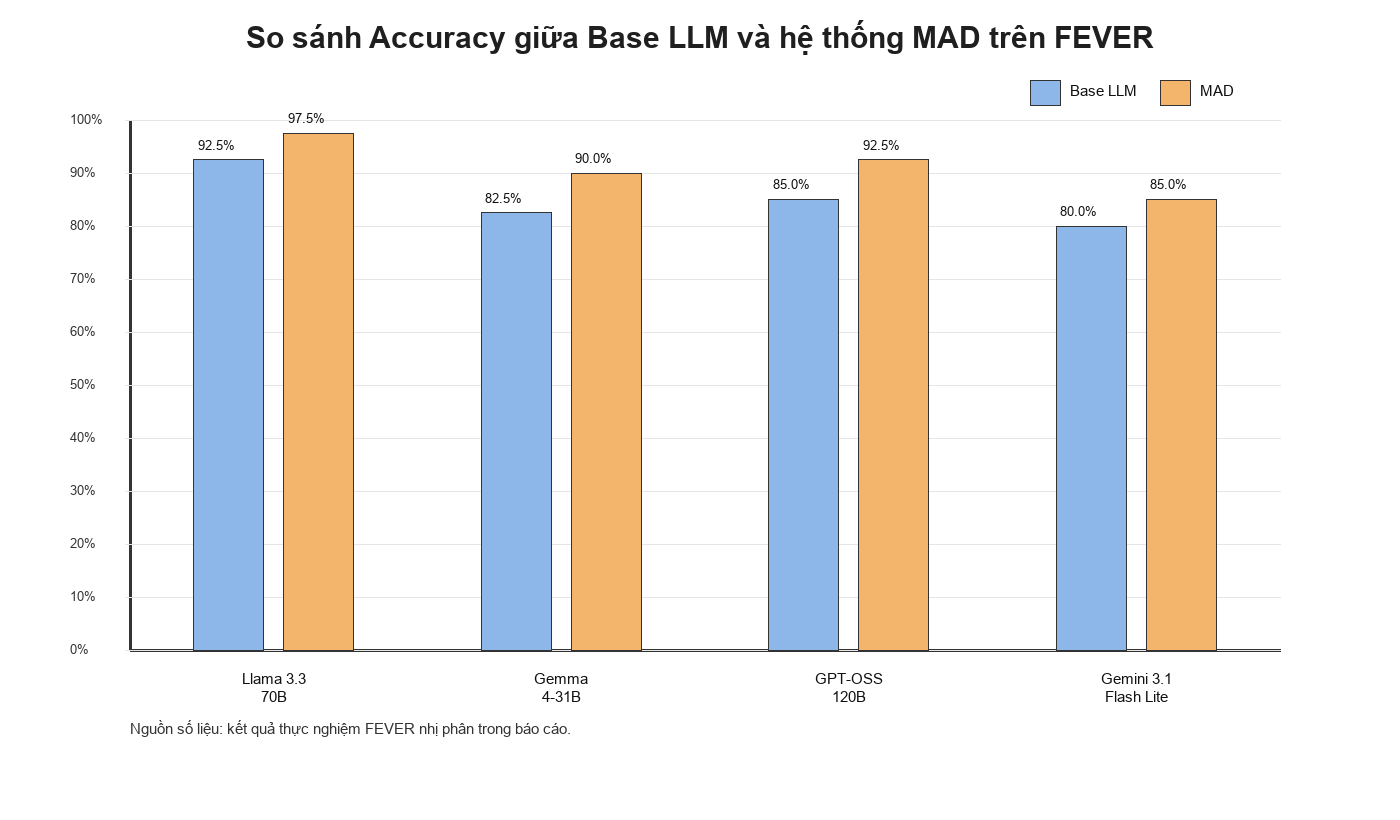
\includegraphics[width=0.95\textwidth]{figures/fever_accuracy_comparison.png}
    \caption{So sánh độ chính xác giữa mô hình nền đơn lẻ và hệ thống MAD trên FEVER}
    \label{fig:fever-accuracy-comparison}
\end{figure}

\section{Phân tích các ca thất bại tiêu biểu}

Bên cạnh kết quả tổng hợp, việc phân tích các ca thất bại có vai trò quan trọng vì nó cho thấy hệ thống sai theo cách nào. Trong kiểm chứng thông tin, không phải mọi lỗi sai đều có cùng ý nghĩa. Có trường hợp hệ thống sai vì thiếu bằng chứng, có trường hợp sai vì mô hình không tuân thủ định dạng, có trường hợp sai so với nhãn dữ liệu nhưng lập luận lại phản ánh một cách hiểu nghiêm ngặt hơn về nhận định. Vì vậy, phân tích định tính giúp đánh giá hệ thống sâu hơn các chỉ số tổng hợp.

Một ca đáng chú ý là nhận định ``Frank Ocean was in a poll''. Trong dữ liệu FEVER, nhận định này được gán nhãn đúng. Tuy nhiên, MAD có xu hướng đánh giá thấp nhận định vì phân biệt giữa việc một nghệ sĩ xuất hiện trong một danh sách do biên tập viên chọn và việc xuất hiện trong một cuộc thăm dò ý kiến theo nghĩa chặt. Tác tử phản biện lập luận rằng các ví dụ như danh sách ảnh hưởng hoặc bảng xếp hạng biên tập không nhất thiết là ``poll''. Tác tử phán quyết nghiêng về cách hiểu nghiêm ngặt này và cho điểm thấp. Đây là một thất bại theo nhãn dữ liệu, nhưng cũng là một ví dụ cho thấy hệ thống có khả năng phát hiện mơ hồ thuật ngữ.

Một ca khác liên quan tới nhận định về Hotel Transylvania 2, trong đó nhận định yêu cầu xác nhận một diễn viên đóng vai cụ thể. Nguồn Wikipedia có thể xác nhận diễn viên tham gia bộ phim nhưng không ghi rõ tên nhân vật trong đoạn ngữ cảnh được cung cấp. Trong trường hợp này, MAD đánh giá nhận định là không đủ bằng chứng thay vì suy đoán. Nếu nhãn gốc là đúng, hệ thống bị tính là sai. Tuy nhiên, về mặt nguyên tắc kiểm chứng thông tin, đây là hành vi thận trọng: nếu nguồn hiện có không xác nhận chi tiết then chốt, hệ thống không nên tự điền phần còn thiếu.

Một nhóm lỗi khác là lỗi phân tích cú pháp hoặc đầu ra có cấu trúc, thường xuất hiện nhiều hơn với các mô hình nhỏ. Trong các trường hợp này, quá trình tranh luận có thể đã diễn ra, nhưng tác tử phán quyết không trả về JSON đúng định dạng hoặc thiếu trường bắt buộc. Dù hệ thống có bộ phân tích cú pháp nhiều tầng, vẫn có trường hợp không cứu được đầu ra. Nhóm lỗi này cho thấy một thách thức thực tế của hệ thống LLM: không chỉ cần suy luận đúng, mà còn cần tuân thủ giao thức đầu ra ổn định để quy trình xử lý có thể xử lý tự động.

Các ca thất bại có thể được phân loại thành một số nhóm. Nhóm thứ nhất là lỗi do bằng chứng không đủ chi tiết. Nhóm thứ hai là lỗi do nhận định hoặc nhãn dữ liệu mơ hồ. Nhóm thứ ba là lỗi suy luận định lượng hoặc phạm vi, ví dụ nhầm giữa một tập hợp tổng và một tập hợp con. Nhóm thứ tư là lỗi kỹ thuật liên quan tới định dạng đầu ra. Việc phân loại này giúp xác định hướng cải tiến cụ thể thay vì chỉ nhìn vào số lượng mẫu sai.

\section{Nhận xét chung}

Từ kết quả thực nghiệm, có thể rút ra một số nhận xét. Thứ nhất, hệ thống MAD cải thiện độ chính xác so với mô hình nền đơn lẻ trên nhiều mô hình nền. Điều này cho thấy cách tổ chức suy luận có ảnh hưởng đáng kể tới chất lượng kiểm chứng. Một mô hình khi được hỏi trực tiếp có thể trả lời sai, nhưng khi được đặt trong quy trình có bằng chứng, phản biện và phán quyết tổng hợp, kết quả có thể tốt hơn.

Thứ hai, MAD có xu hướng thận trọng hơn. Hệ thống không dễ dàng xác nhận nhận định là đúng nếu bằng chứng không hỗ trợ trực tiếp. Đây là ưu điểm trong bối cảnh phát hiện tin giả, vì xác nhận sai một thông tin giả có thể gây hậu quả nghiêm trọng. Tuy nhiên, sự thận trọng này cũng có thể dẫn tới âm tính giả, đặc biệt khi ngữ cảnh thiếu một chi tiết nhưng nhận định thực tế là đúng.

Thứ ba, khả năng giải thích là điểm mạnh rõ ràng của MAD. Với mô hình nền đơn lẻ, người dùng thường chỉ nhận được một câu trả lời và một đoạn giải thích ngắn. Với MAD, người dùng có thể xem quá trình tác tử bảo vệ và tác tử phản biện xây dựng lập luận, nguồn nào được trích dẫn và tác tử phán quyết dựa vào điểm nào để kết luận. Điều này làm cho hệ thống phù hợp hơn với các kịch bản cần kiểm tra truy vết, phân tích lỗi hoặc trình bày trước người dùng.

Thứ tư, chi phí vận hành là hạn chế cần cân nhắc. MAD cần nhiều lần gọi mô hình hơn, đặc biệt khi chạy nhiều vòng và có tìm kiếm. Điều này làm tăng thời gian xử lý và chi phí API. Vì vậy, trong ứng dụng thực tế, cần cân nhắc số vòng tranh luận, lựa chọn mô hình, lưu đệm, định tuyến và cơ chế dừng sớm để cân bằng giữa chất lượng và chi phí.

Cuối cùng, kết quả cho thấy hướng tiếp cận đa tác tử không thay thế hoàn toàn nhu cầu cải thiện mô hình nền hoặc dữ liệu bằng chứng. Nếu ngữ cảnh sai hoặc thiếu, hệ thống vẫn có thể kết luận sai. Nếu mô hình nền yếu trong việc tuân thủ JSON, quy trình xử lý vẫn có thể lỗi. Do đó, MAD nên được xem là một kiến trúc tăng cường khả năng kiểm chứng của LLM, chứ không phải giải pháp loại bỏ mọi hạn chế của LLM.
\chapter{Kết luận và hướng phát triển}

\section{Kết luận}

Đồ án đã nghiên cứu và xây dựng một hệ thống phát hiện tin giả dựa trên phương pháp tranh biện đa tác tử. Thay vì sử dụng một mô hình ngôn ngữ đơn lẻ để đưa ra phán quyết trực tiếp, hệ thống tổ chức một quy trình kiểm chứng nhiều bước gồm truy xuất bằng chứng, chấm điểm nguồn, tranh luận giữa các tác tử và tổng hợp phán quyết cuối cùng. Cách tiếp cận này phù hợp với đặc thù của bài toán kiểm chứng thông tin, nơi kết quả cần có bằng chứng, giải thích và khả năng truy vết.

Về mặt kiến trúc, hệ thống đã triển khai các thành phần chính gồm tác tử bảo vệ, tác tử phản biện, bộ đánh giá nguồn, bộ quản lý nhận định và tác tử phán quyết. Tác tử bảo vệ có nhiệm vụ bảo vệ bản tin, tác tử phản biện phản biện và tìm điểm yếu, Bộ đánh giá nguồn đánh giá chất lượng nguồn, bộ quản lý nhận định quản lý các nhận định qua nhiều vòng, còn Tác tử phán quyết tổng hợp toàn bộ quá trình để đưa ra \texttt{truth\_score}. Các thành phần này được điều phối bằng LangGraph thông qua trạng thái MAD, cho phép hệ thống duy trì trạng thái qua nhiều vòng tranh luận.

Về mặt vận hành, hệ thống hỗ trợ hai chế độ. chế độ tìm kiếm cho phép hệ thống tự tìm kiếm bằng chứng từ bên ngoài thông qua Tavily hoặc Wikipedia. chế độ không tìm kiếm cho phép hệ thống suy luận trong phạm vi ngữ cảnh được cung cấp sẵn, phù hợp với bộ đánh giá FEVER. Việc hỗ trợ hai chế độ giúp hệ thống vừa có khả năng trình diễn trong môi trường mở, vừa có khả năng đánh giá trong môi trường kiểm soát.

Về mặt thực nghiệm, kết quả trên FEVER cho thấy hệ thống MAD cải thiện độ chính xác so với mô hình nền đơn lẻ trên nhiều mô hình nền. Ngoài cải thiện định lượng, hệ thống còn tạo ra lịch sử tranh luận và phần giải thích, giúp quá trình kiểm chứng minh bạch hơn. Các phân tích trường hợp nghiên cứu cho thấy MAD có xu hướng thận trọng hơn, ít suy đoán khi bằng chứng thiếu chi tiết, đồng thời có khả năng phát hiện một số vấn đề như đánh tráo khái niệm hoặc nhận định mơ hồ.

Nhìn chung, đồ án cho thấy việc tổ chức LLM thành một quy trình nhiều tác tử có thể nâng cao chất lượng kiểm chứng thông tin so với cách hỏi trực tiếp. Đóng góp chính của hệ thống không chỉ nằm ở kết quả dự đoán, mà còn ở cấu trúc kiểm chứng có thể giải thích, phân tích và mở rộng.

\section{Hạn chế}

Mặc dù đạt được một số kết quả tích cực, hệ thống vẫn còn các hạn chế. Hạn chế đầu tiên là chi phí thời gian và token. So với mô hình nền đơn lẻ, MAD cần nhiều lần gọi mô hình hơn vì phải chạy nhiều tác tử và nhiều vòng tranh luận. Điều này làm thời gian xử lý trung bình trên mỗi mẫu cao hơn, đặc biệt với các mô hình lớn hoặc khi chế độ tìm kiếm sử dụng nhiều truy vấn.

Hạn chế thứ hai là hệ thống vẫn phụ thuộc vào chất lượng mô hình nền. Nếu mô hình không đủ mạnh trong suy luận, không tuân thủ định dạng đầu ra hoặc dễ lặp lại lập luận, chất lượng của toàn bộ luồng xử lý sẽ bị ảnh hưởng. Các cơ chế phân tích cú pháp nhiều tầng và thử lại chỉ giảm một phần lỗi kỹ thuật, không thể thay thế hoàn toàn năng lực của mô hình.

Hạn chế thứ ba là chất lượng bằng chứng ảnh hưởng trực tiếp tới kết quả. Trong chế độ tìm kiếm, nếu công cụ tìm kiếm không tìm được nguồn phù hợp hoặc nguồn có nội dung không đầy đủ, các tác tử có thể lập luận trên nền tảng yếu. Trong chế độ không tìm kiếm, nếu ngữ cảnh đầu vào thiếu chi tiết quan trọng, hệ thống có thể kết luận thận trọng nhưng sai so với nhãn gốc.

Hạn chế thứ tư là hệ thống hiện tập trung vào văn bản. Các dạng tin giả hiện đại có thể kết hợp hình ảnh, video, âm thanh hoặc ảnh chụp màn hình. Hệ thống chưa xử lý trực tiếp các nguồn đa phương tiện này, nên phạm vi ứng dụng vẫn còn giới hạn.

Hạn chế cuối cùng nằm ở giao diện và mức độ hoàn thiện sản phẩm. Lõi luồng xử lý và các kịch bản thực nghiệm đã thể hiện được ý tưởng chính của đồ án, nhưng để trở thành một ứng dụng hoàn chỉnh, hệ thống cần được đồng bộ thêm về giao diện, xử lý lỗi người dùng, lưu đệm, quản lý phiên chạy và triển khai thực tế.

\section{Hướng phát triển}

Hướng phát triển đầu tiên là tối ưu hiệu năng và chi phí. Hệ thống có thể bổ sung cơ chế dừng sớm nếu tranh luận đã hội tụ, giảm số vòng trong các nhận định đơn giản hoặc dùng mô hình nhỏ cho các bước phụ và mô hình lớn cho tác tử phán quyết. Ngoài ra, lưu đệm kết quả tìm kiếm và lưu đệm chấm điểm nguồn cũng có thể giảm chi phí khi nhiều nhận định liên quan tới cùng chủ đề.

Hướng phát triển thứ hai là cải thiện đầu ra có cấu trúc. Thay vì chỉ dựa vào chỉ dẫn và bộ phân tích cú pháp thủ công, hệ thống có thể sử dụng kiểm tra theo lược đồ, gọi hàm hoặc gọi công cụ để đảm bảo đầu ra của các tác tử luôn có định dạng hợp lệ. Điều này đặc biệt quan trọng khi chạy bộ đánh giá lớn hoặc sử dụng các mô hình nhỏ có khả năng tuân thủ định dạng chưa ổn định.

Hướng phát triển thứ ba là mở rộng cơ chế đánh giá và kiểm soát chất lượng lập luận. Hệ thống có thể tích hợp rõ hơn một bộ đánh giá trung gian để đánh giá từng nhận định sau mỗi vòng, loại bỏ nhận định không có bằng chứng, đánh dấu nhận định đã được giải quyết và hướng dẫn vòng tranh luận tiếp theo. Điều này giúp giảm tranh luận lặp lại và làm cho luồng xử lý chặt chẽ hơn.

Hướng phát triển thứ tư là mở rộng bộ dữ liệu đánh giá. Ngoài FEVER, hệ thống có thể được thử nghiệm sâu hơn trên GossipCop, TruthfulQA hoặc các bộ dữ liệu kiểm chứng thông tin đa ngôn ngữ. Việc đánh giá trên nhiều loại dữ liệu giúp kiểm tra xem MAD hoạt động tốt với nhận định bách khoa, tin giải trí, tin chính trị hay câu hỏi gây hiểu lầm phổ biến ở mức nào.

Hướng phát triển thứ năm là hỗ trợ kiểm chứng đa ngôn ngữ và đa phương tiện. Với tiếng Việt, hệ thống cần cải thiện truy vấn, nguồn tin và khả năng xử lý ngữ cảnh bản địa. Với dữ liệu đa phương tiện, hệ thống có thể bổ sung nhận dạng ký tự quang học, phân tích ảnh hoặc trích xuất thông tin từ video trước khi đưa vào quy trình MAD. Khi đó, MAD có thể trở thành lớp suy luận và tranh luận phía trên nhiều loại bộ trích xuất bằng chứng khác nhau.

Tóm lại, hướng phát triển lâu dài của hệ thống là chuyển từ một nguyên mẫu nghiên cứu sang một nền tảng kiểm chứng thông tin có khả năng mở rộng. Kiến trúc tranh biện đa tác tử trong đồ án tạo nền tảng cho hướng đi này vì nó tách biệt rõ các thành phần: thu thập bằng chứng, đánh giá nguồn, tranh luận, quản lý lập luận và phán quyết.

\begin{thebibliography}{99}

\bibitem{vosoughi2018spread}
S. Vosoughi, D. Roy, and S. Aral, ``The spread of true and false news online,'' \textit{Science}, vol. 359, no. 6380, pp. 1146--1151, 2018.

\bibitem{thorne2018fever}
J. Thorne, A. Vlachos, C. Christodoulopoulos, and A. Mittal, ``FEVER: a large-scale dataset for fact extraction and verification,'' in \textit{Proceedings of NAACL-HLT}, 2018.

\bibitem{lewis2020rag}
P. Lewis et al., ``Retrieval-augmented generation for knowledge-intensive NLP tasks,'' in \textit{Advances in Neural Information Processing Systems}, 2020.

\bibitem{irving2018debate}
G. Irving, P. Christiano, and D. Amodei, ``AI safety via debate,'' arXiv preprint arXiv:1805.00899, 2018.

\bibitem{du2023improving}
Y. Du et al., ``Improving factuality and reasoning in language models through multiagent debate,'' arXiv preprint arXiv:2305.14325, 2023.

\bibitem{langgraph}
LangChain, ``LangGraph documentation,'' truy cập năm 2026. [Trực tuyến]. Available: https://langchain-ai.github.io/langgraph/

\bibitem{gradio}
Gradio, ``Gradio documentation,'' truy cập năm 2026. [Trực tuyến]. Available: https://www.gradio.app/docs

\end{thebibliography}
\end{document}




























